Este capítulo cubre el análisis del sistema de información a desarrollar, haciendo uso del lenguaje de modelado UML.

\section{Modelo de Casos de Uso}
\label{sec:usecases}
Se asume que los casos de uso en los que interviene el rol de comercial pueden ser igualmente realizados por el rol de administrador, al disponer este de permisos equivalentes o superiores dentro del sistema. Por este motivo, y con el objetivo de mejorar la claridad del modelo, se ha optado por representar únicamente el rol de comercial en los casos de uso compartidos, evitando redundancias innecesarias en los diagramas. No obstante, en aquellos casos en los que existen funcionalidades exclusivas del rol de administrador, este se ha representado explícitamente.

Este enfoque es coherente con el modelado de casos de uso, en el que los actores representan roles que interactuan con el sistema \citep[Ch.~4]{sommerville}.

\bigskip

En la versión actual del proyecto, los diagramas asociados a \texttt{M1}, \texttt{M2}, \texttt{M3} y \texttt{M4} deben interpretarse como módulos ya implementados y operativos. El caso de \texttt{M5} pasa a una situación intermedia: existe ya una implementación funcional de fichas del salón, alta, edición y borrado de servicios, ficha técnica, plantillas reutilizables, sugerencias derivadas y borradores técnicos editables por servicio, pero el diagrama sigue recogiendo además capacidades aún no construidas, como el envío real del correo a cliente final. En \texttt{M6} ya existe un núcleo interno de promociones, segmentación, formaciones, notificaciones, recordatorios y descuentos promocionales aplicados al pedido, aunque la mensajería externa sigue siendo planificación futura. El diagrama de \texttt{M8} conserva valor de análisis y planificación, mientras que \texttt{M7} dispone ya de auditoría administrativa, configuración global de rate limiting, resumen operativo, integraciones de soporte, soporte técnico/PWA y un primer subsistema persistente para integraciones empresariales, operaciones de intercambio y propuestas de pedido a proveedor.

\newpage{\ }
\subsection{Casos de Uso M1.}

En este módulo se han representado los casos de uso relacionados con la gestión de acceso, alta y autorización de usuarios.

\begin{figure}[H]
    \centering
    \includegraphics[width=0.8\textwidth]{./figures/UML/CasosDeUso/M1_CasosDeUso.pdf}
    \caption{Casos de Uso M1. Gestión de acceso, alta y autorización de usuarios}
    \label{fig:M1_CasosDeUso}
\end{figure}

\newpage{\ }
\subsection{Casos de Uso M2.}

En este módulo se han representado los casos de uso relacionados con la gestión comercial y clientes.

\begin{figure}[H]
    \centering
    \includegraphics[width=0.8\textwidth]{./figures/UML/CasosDeUso/M2_CasosDeUso.pdf}
    \caption{Casos de Uso M2. Gestión comercial y clientes}
    \label{fig:M2_CasosDeUso}
\end{figure}

\newpage{\ }
\subsection{Casos de Uso M3.}

En este módulo se han representado los casos de uso relacionados con el catálogo, productos y coloración.

\begin{figure}[H]
    \centering
    \includegraphics[width=0.8\textwidth]{./figures/UML/CasosDeUso/M3_CasosDeUso.pdf}
    \caption{Casos de Uso M3. Catálogo, productos y coloración}
    \label{fig:M3_CasosDeUso}
\end{figure}

\newpage{\ }
\subsection{Casos de Uso M4.}

En este módulo se han representado los casos de uso relacionados con los pedidos, entregas y cobros.

\begin{figure}[H]
    \centering
    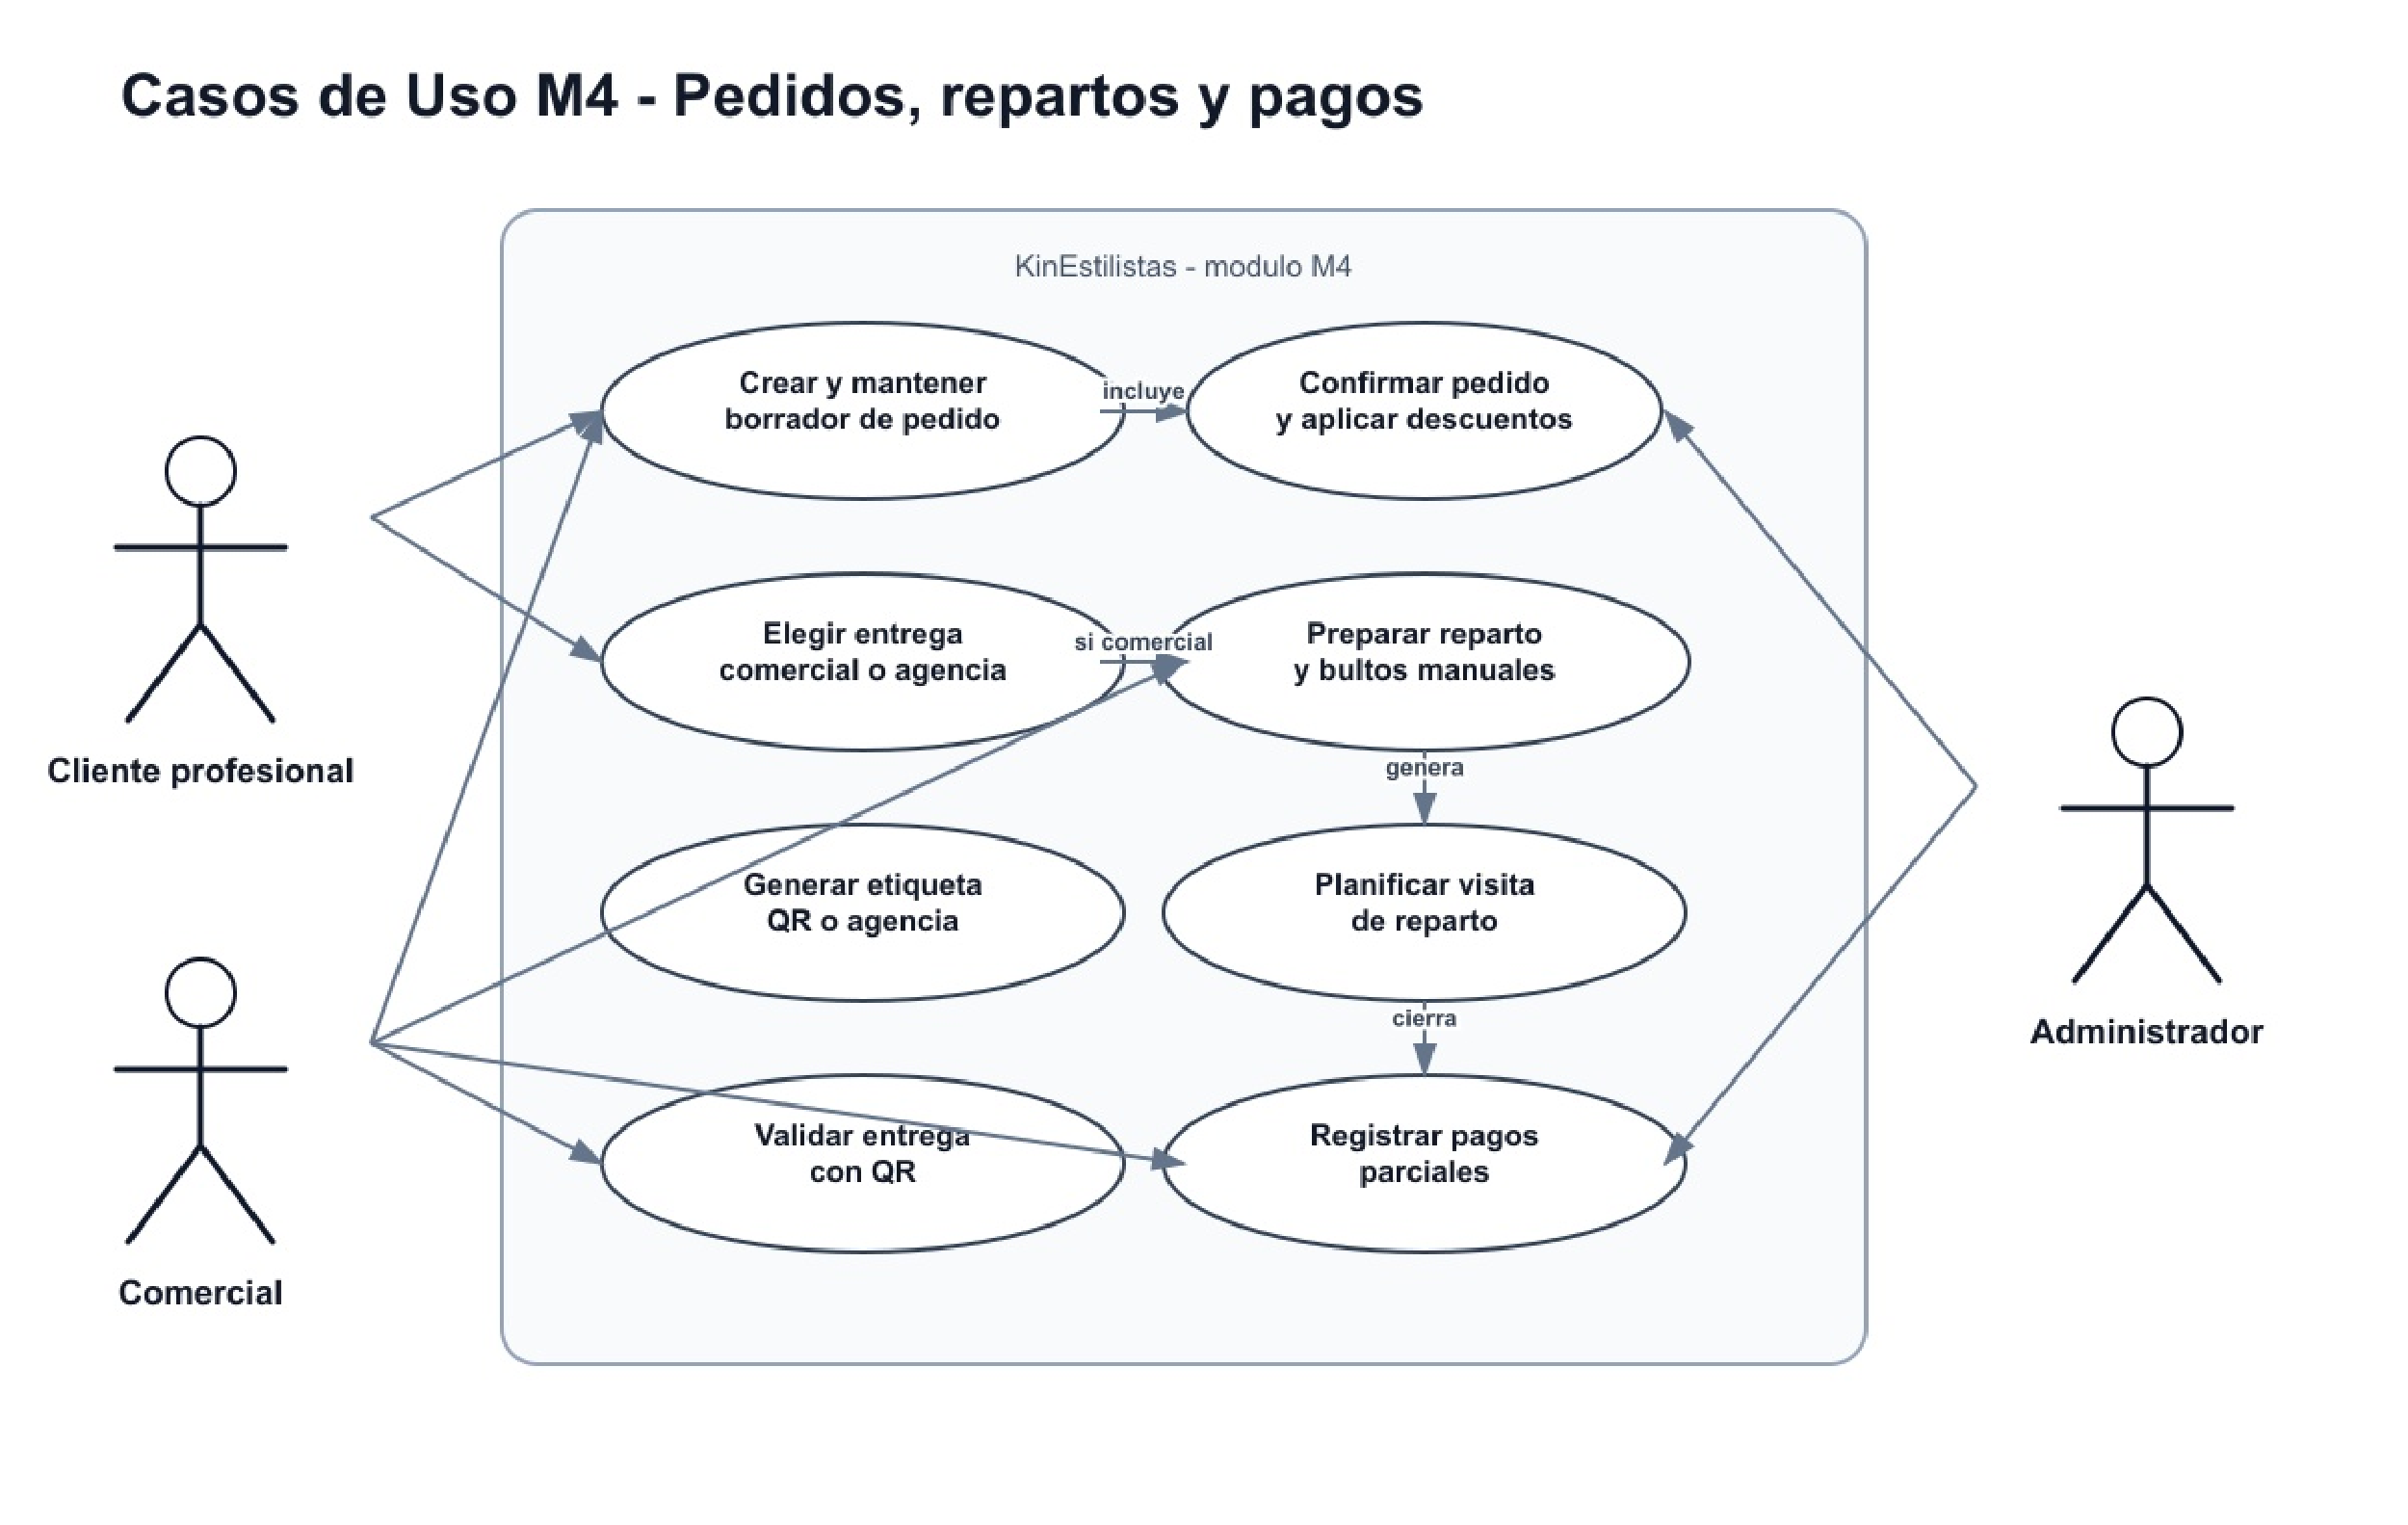
\includegraphics[width=0.8\textwidth]{./figures/UML/CasosDeUso/M4_CasosDeUso.pdf}
    \caption{Casos de Uso M4. Pedidos, entregas y cobros}
    \label{fig:M4_CasosDeUso}
\end{figure}

\newpage{\ }
\subsection{Casos de Uso M5.}

En este módulo se han representado los casos de uso relacionados con la gestión interna de peluquerías. En la implementación actual ya existe un subconjunto operativo de estos casos de uso, centrado en fichas técnicas internas, historial de servicios con mantenimiento posterior, plantillas reutilizables, uso de productos con tonalidad concreta cuando procede, galería visual del resultado final, sugerencias derivadas y preparación asistida de borradores de correo técnico.

\begin{figure}[H]
    \centering
    \includegraphics[width=0.8\textwidth]{./figures/UML/CasosDeUso/M5_CasosDeUso.pdf}
    \caption{Casos de Uso M5. Gestión interna de peluquerías}
    \label{fig:M5_CasosDeUso}
\end{figure}

\newpage{\ }
\subsection{Casos de Uso M6.}

En este módulo se han representado los casos de uso relacionados con promociones, notificaciones y formaciones. La implementación actual cubre ya el flujo interno principal: administración de promociones, segmentación manual, publicación de formaciones, notificaciones dentro de la aplicación, recordatorios personales y aplicación de descuentos promocionales sobre pedidos. Las integraciones multicanal externas siguen formando parte de la evolución futura.

\begin{figure}[H]
    \centering
    \includegraphics[width=0.8\textwidth]{./figures/UML/CasosDeUso/M6_CasosDeUso.pdf}
    \caption{Casos de Uso M6. Promociones, notificaciones y formaciones}
    \label{fig:M6_CasosDeUso}
\end{figure}

\newpage{\ }
\subsection{Casos de Uso M7.}

En este módulo se han representado los casos de uso relacionados con administración e integraciones. En la implementación real, la parte hoy desplegada de este bloque cubre auditoría, configuración global de rate limiting, resumen operativo transversal, inventario operativo de integraciones de soporte, soporte transversal a servicios externos, soporte técnico de compatibilidad/PWA, registro persistente de integraciones empresariales, operaciones de exportación o sincronización y generación de propuestas de pedido a proveedor.

\begin{figure}[H]
    \centering
    \includegraphics[width=0.8\textwidth]{./figures/UML/CasosDeUso/M7_CasosDeUso.pdf}
    \caption{Casos de Uso M7. Administración e integraciones}
    \label{fig:M7_CasosDeUso}
\end{figure}

\newpage{\ }
\subsection{Casos de Uso M8.}

En este módulo se han representado los casos de uso relacionados con funcionalidades adicionales. Dado que las funcionalidades recogidas en este módulo no forman parte del alcance principal de la versión actualmente implementada del sistema, el diagrama asociado debe interpretarse como una representación conceptual de posibles extensiones futuras de la plataforma.

\begin{figure}[H]
    \centering
    \includegraphics[width=0.8\textwidth]{./figures/UML/CasosDeUso/M8_CasosDeUso.pdf}
    \caption{Casos de Uso M8. Funcionalidades adicionales}
    \label{fig:M8_CasosDeUso}
\end{figure}


\section{Modelo Conceptual}
\label{sec:conceptualmodel}
A partir de los requisitos de información definidos en la \autoref{sec:InformationRequirements}, se ha
elaborado el modelo conceptual de datos correspondiente. Este modelo describe las principales entidades de información que intervienen en la gestión de
usuarios del sistema, así como sus atributos y relaciones.

Para mayor legibilidad, el modelo conceptual se representa mediante varios diagramas de clases UML separados por módulos. En ellos se se identifican las clases del dominio, los atributos que describen la información gestionada y las relaciones existentes entre dichas clases.

% ------------------------------------------------------------------------------
\subsection{Modelo conceptual de datos M1}
% ------------------------------------------------------------------------------
La \autoref{fig:mcd-m1} muestra el modelo conceptual correspondiente al módulo de gestión de acceso, alta y autorización de usuarios.

% \begin{figure}[H]
%     \centering
%     \includegraphics[width=\textwidth]{figures/MCD/M1_ModeloConceptual.pdf}
%     \caption{Modelo conceptual de datos del módulo M1.}
%     \label{fig:mcd-m1}
% \end{figure}

\subsubsection{Clase Usuario}

La clase \textit{Usuario} representa a cada persona o entidad con acceso al sistema. En ella se almacena la información necesaria para identificar al usuario, gestionar su autenticación y determinar su rol dentro de la aplicación.

\textbf{Atributos}

\begin{itemize}

      \item \textit{id}
            Identificador único del usuario.
      \item \textit{email}
            Dirección de correo electrónico utilizada para la autenticación.
      \item \textit{password\_hash}
            Contraseña cifrada del usuario.
      \item \textit{name}
            Nombre completo del usuario.
      \item \textit{phone}
            Número de teléfono de contacto.
      \item \textit{company}
            Empresa o entidad a la que pertenece el usuario.
      \item \textit{role}
            Rol asignado al usuario dentro del sistema.
      \item \textit{status}
            Estado actual de la cuenta de usuario.
      \item \textit{profile\_image\_url}
            Dirección de la imagen de perfil del usuario.
      \item \textit{last\_login\_at}
            Fecha y hora del último acceso al sistema.
      \item \textit{created\_at}
            Fecha de creación de la cuenta.
      \item \textit{updated\_at}
            Fecha de última actualización de la información del usuario.

\end{itemize}

\textbf{Restricciones textuales}

\begin{itemize}

      \item \textbf{RT-U1 — Email único}
            Cada usuario debe tener una dirección de correo electrónico única dentro del sistema.
      \item \textbf{RT-U2 — Rol obligatorio}
            Todo usuario debe tener asignado un rol válido dentro del sistema.
      \item \textbf{RT-U3 — Estado válido de usuario}
            El estado de un usuario solo puede tomar valores definidos por el sistema.
      \item \textbf{RT-U4 — Acceso solo para usuarios activos}
            Un usuario únicamente puede autenticarse en el sistema si su estado es \textit{active}.
      \item \textbf{RT-U5 — Empresa obligatoria para clientes}
            Si un usuario tiene asignado el rol cliente, el atributo \textit{company} no puede ser nulo ni vacío.
      \item \textbf{RT-U6 — Fecha de creación obligatoria}
            Todo usuario debe registrar la fecha de creación de la cuenta.
      \item \textbf{RT-U7 — Consistencia temporal del último acceso}
            Si el atributo \textit{last\_login\_at} tiene valor, este debe ser posterior o igual a la fecha de creación de la cuenta.

\end{itemize}

\subsubsection{Clase Rol}

La clase \textit{Rol} define los distintos perfiles de acceso existentes en el sistema. Los roles permiten determinar las funcionalidades a las que puede acceder cada usuario.

\textbf{Atributos}

\begin{itemize}

      \item \textit{id}
            Identificador del rol.
      \item \textit{code}
            Código identificativo del rol.
      \item \textit{name}
            Nombre del rol.
      \item \textit{description}
            Descripción del rol.

\end{itemize}

\textbf{Restricciones textuales}

\begin{itemize}

      \item \textbf{RT-RO1 — Identificador único de rol}
            Cada rol del sistema debe tener un identificador único, así como un código y un nombre únicos.

\end{itemize}

\subsubsection{Clase Solicitud de registro}

La clase \textit{Solicitud de registro} representa las solicitudes de alta realizadas por usuarios que desean acceder al sistema y que deben ser revisadas por un administrador.

\textbf{Atributos}

\begin{itemize}

      \item \textit{id}
            Identificador de la solicitud.
      \item \textit{email}
            Correo electrónico del solicitante.
      \item \textit{password\_hash}
            Contraseña cifrada propuesta por el solicitante.
      \item \textit{name}
            Nombre del solicitante.
      \item \textit{phone}
            Teléfono de contacto.
      \item \textit{company}
            Empresa asociada al solicitante.
      \item \textit{requested\_role}
            Rol solicitado por el usuario.
      \item \textit{status}
            Estado actual de la solicitud.
      \item \textit{request\_source}
            Origen de la solicitud de registro.
      \item \textit{requested\_at}
            Fecha en la que se realiza la solicitud.
      \item \textit{reviewed\_at}
            Fecha en la que se revisa la solicitud.
      \item \textit{reviewed\_by}
            Usuario que revisa la solicitud.
      \item \textit{rejection\_reason}
            Motivo del rechazo de la solicitud.
      \item \textit{created\_user}
            Usuario creado a partir de la solicitud aprobada.

\end{itemize}

\textbf{Restricciones textuales}

\begin{itemize}

      \item \textbf{RT-R1 — Estado obligatorio en solicitudes de registro}
            Toda solicitud de registro debe tener un estado definido.
      \item \textbf{RT-R2 — Solicitudes pendientes no revisadas}
            Si una solicitud de registro tiene estado \textit{pending}, no puede existir información de revisión asociada.
      \item \textbf{RT-R3 — Solicitudes revisadas deben registrar revisión}
            Si una solicitud tiene estado \textit{approved} o \textit{rejected}, debe registrarse la información de revisión correspondiente.
      \item \textbf{RT-R4 — Motivo obligatorio en solicitudes rechazadas}
            Si una solicitud de registro es rechazada, debe registrarse el motivo del rechazo.
      \item \textbf{RT-R5 — Creación de usuario tras aprobación}
            Si una solicitud de registro es aprobada, debe generarse una cuenta de usuario asociada.
      \item \textbf{RT-R6 — Rol solicitado válido}
            El rol solicitado en una solicitud de registro debe corresponder a uno de los roles existentes en el sistema.

\end{itemize}

\subsubsection{Clase Registro de administración de usuarios}

Esta clase permite registrar las acciones administrativas realizadas sobre las cuentas de usuario, proporcionando trazabilidad sobre los cambios efectuados en el sistema.

\textbf{Atributos}

\begin{itemize}

      \item \textit{id}
            Identificador del registro.
      \item \textit{target\_user}
            Usuario sobre el que se realiza la acción.
      \item \textit{performed\_by}
            Usuario que realiza la acción administrativa.
      \item \textit{action\_type}
            Tipo de acción administrativa realizada.
      \item \textit{previous\_status}
            Estado previo del usuario.
      \item \textit{new\_status}
            Nuevo estado del usuario.
      \item \textit{previous\_role}
            Rol previo del usuario.
      \item \textit{new\_role}
            Nuevo rol asignado al usuario.
      \item \textit{reason}
            Motivo de la acción administrativa.
      \item \textit{notes}
            Información adicional asociada a la acción.
      \item \textit{created\_at}
            Fecha en la que se registra la acción.

\end{itemize}

\textbf{Restricciones textuales}

\begin{itemize}

      \item \textbf{RT-L1 — Acción administrativa obligatoria}
            Todo registro debe indicar el tipo de acción realizada.
      \item \textbf{RT-L2 — Usuario objetivo obligatorio}
            Toda acción administrativa debe referirse a un usuario existente en el sistema.
      \item \textbf{RT-L3 — Actor de la acción obligatorio}
            Toda acción administrativa debe registrar el usuario que realizó la acción.
      \item \textbf{RT-L4 — Consistencia en cambios de rol}
            Si la acción corresponde a un cambio de rol, deben registrarse el rol anterior y el nuevo rol.
      \item \textbf{RT-L5 — Consistencia en cambios de estado}
            Si la acción corresponde a un cambio de estado, deben registrarse el estado anterior y el nuevo estado.
      \item \textbf{RT-G3 — Registro obligatorio de acciones administrativas}
            Toda acción administrativa que modifique el estado o el rol de un usuario debe quedar registrada.

\end{itemize}

\subsubsection{Clase Registro de acceso}

La clase \textit{Registro de acceso} almacena los eventos relacionados con el acceso al sistema, incluyendo intentos de autenticación, creación de sesiones y eventos de cierre o expiración.

\textbf{Atributos}

\begin{itemize}

      \item \textit{id}
            Identificador del registro de acceso.
      \item \textit{user}
            Usuario asociado al evento de acceso.
      \item \textit{email\_attempted}
            Correo electrónico utilizado en el intento de acceso.
      \item \textit{event\_type}
            Tipo de evento de acceso.
      \item \textit{result}
            Resultado del intento de acceso.
      \item \textit{failure\_reason}
            Motivo del fallo en caso de error.
      \item \textit{session\_token}
            Identificador de la sesión asociada.
      \item \textit{ip\_address}
            Dirección IP desde la que se realizó el acceso.
      \item \textit{user\_agent}
            Información del navegador o dispositivo utilizado.
      \item \textit{created\_at}
            Fecha y hora del evento de acceso.
      \item \textit{revoked\_at}
            Fecha de revocación de la sesión.
      \item \textit{expires\_at}
            Fecha de expiración de la sesión.

\end{itemize}

\textbf{Restricciones textuales}

\begin{itemize}

      \item \textbf{RT-A1 — Todo registro de acceso debe tener tipo de evento}
            Cada registro debe indicar el tipo de evento correspondiente.
      \item \textbf{RT-A2 — Todo registro de acceso debe tener resultado}
            Cada registro debe indicar el resultado del evento.
      \item \textbf{RT-A3 — Todo registro de acceso debe registrar fecha y hora}
            Cada registro debe contener el instante en que se produjo el evento.
      \item \textbf{RT-A4 — Los eventos fallidos deben registrar el motivo}
            Si el resultado de un evento es fallido, debe registrarse el motivo.
      \item \textbf{RT-A5 — Los eventos de login correcto pueden generar sesión}
            Si el evento corresponde a un acceso correcto, el sistema puede registrar una sesión.
      \item \textbf{RT-A6 — Los eventos de revocación deben referirse a una sesión}
            Los eventos de revocación deben asociarse a una sesión.
      \item \textbf{RT-A7 — Los eventos de expiración deben referirse a una sesión}
            Los eventos de expiración deben asociarse a una sesión.
      \item \textbf{RT-A8 — Coherencia entre usuario y credencial intentada}
            Debe existir al menos un identificador de usuario o un correo utilizado en el intento de acceso.
      \item \textbf{RT-A9 — Coherencia temporal de expiración}
            Si existe una fecha de expiración de sesión, esta debe ser posterior al evento.
      \item \textbf{RT-A10 — Coherencia temporal de revocación}
            Si existe una fecha de revocación, esta debe ser posterior o igual al evento.
      \item \textbf{RT-A11 — Los eventos de cierre o invalidación deben asociarse a una sesión}
            Los eventos de cierre, revocación o expiración deben estar asociados a una sesión.
      \item \textbf{RT-G2 — Invalidación de sesiones en usuarios bloqueados}
            Si el estado de un usuario pasa a \textit{blocked}, cualquier sesión activa debe ser invalidada.

\end{itemize}

% ------------------------------------------------------------------------------
\subsection{Modelo conceptual de datos M2}
% ------------------------------------------------------------------------------

La \autoref{fig:mcd-m2} muestra el modelo conceptual correspondiente al módulo de gestión comercial y clientes.

% \begin{figure}[H]
%     \centering
%     \includegraphics[width=\textwidth]{figures/MCD/M2_ModeloConceptual.pdf}
%     \caption{Modelo conceptual de datos del módulo M2.}
%     \label{fig:mcd-m2}
% \end{figure}

\subsubsection{Clase Cliente}

La clase \textit{Cliente} representa a cada establecimiento profesional atendido por el distribuidor. En ella se almacena la información necesaria para identificar al cliente como entidad comercial, registrar los datos propios del establecimiento, mantener su vinculación con el usuario de acceso correspondiente dentro del sistema y facilitar la consulta de la información de contacto, localización y disponibilidad horaria necesaria para la planificación de visitas y rutas comerciales.

\textbf{Atributos}

\begin{itemize}

      \item \textit{id}
            Identificador único del cliente.
      \item \textit{name}
            Nombre del establecimiento o peluquería.
      \item \textit{contact\_name}
            Nombre de la persona de contacto del establecimiento.
      \item \textit{tax\_id}
            Identificador fiscal del cliente.
      \item \textit{address}
            Dirección del establecimiento.
      \item \textit{city}
            Localidad o ciudad del cliente.
      \item \textit{postal\_code}
            Código postal del establecimiento.
      \item \textit{province}
            Provincia o zona geográfica del cliente.
      \item \textit{linked\_user}
            Usuario asociado al cliente dentro del sistema.
      \item \textit{lat}
            Coordenada de latitud del establecimiento.
      \item \textit{lng}
            Coordenada de longitud del establecimiento.
      \item \textit{visit\_window\_start\_time}
            Hora de inicio de la franja admitida para visitas comerciales.
      \item \textit{visit\_window\_end\_time}
            Hora de fin de la franja admitida para visitas comerciales.
      \item \textit{notes}
            Observaciones o notas comerciales asociadas al cliente.
      \item \textit{created\_at}
            Fecha de creación del registro del cliente.
      \item \textit{updated\_at}
            Fecha de última actualización de la información del cliente.

\end{itemize}

\textbf{Restricciones textuales}

\begin{itemize}

      \item \textbf{RT-C1 — Identificación obligatoria del cliente}
            Todo cliente debe disponer de información suficiente para su identificación dentro del sistema.
      \item \textbf{RT-C2 — Vinculación obligatoria con usuario}
            Todo cliente debe estar asociado a un único usuario del sistema que represente su cuenta de acceso a la plataforma.
      \item \textbf{RT-C3 — Correspondencia entre cliente y usuario cliente}
            Todo usuario con rol cliente debe corresponder a una única entidad \textit{Cliente} dentro del sistema.
      \item \textbf{RT-C4 — Consistencia de geolocalización}
            Si el cliente dispone de latitud o longitud registradas, ambas coordenadas deben estar informadas conjuntamente.
      \item \textbf{RT-C5 — Coherencia de ventana de visita}
            Si se define una franja horaria de visita para el cliente, la hora de fin debe ser posterior a la hora de inicio.
      \item \textbf{RT-C6 — Coherencia temporal del registro del cliente}
            Si el atributo \textit{updated\_at} tiene valor, este debe ser posterior o igual a la fecha de creación del cliente.
      \item \textbf{RT-C7 — Identificación fiscal consistente}
            Si un cliente dispone de un identificador fiscal, este debe ser válido.

\end{itemize}

\subsubsection{Clase Comercial}

La clase \textit{Comercial} representa el perfil operativo de un usuario con funciones comerciales dentro del sistema. Su finalidad es complementar la información general del usuario con datos específicos de trabajo de campo, tales como su territorio, los parámetros base de la jornada y la configuración utilizada para calcular rutas diarias.

\textbf{Atributos}

\begin{itemize}

      \item \textit{id}
            Identificador único del comercial.
      \item \textit{user}
            Usuario del sistema asociado al perfil comercial.
      \item \textit{employee\_code}
            Código interno del comercial, cuando exista.
      \item \textit{territory}
            Zona o territorio comercial asignado.
      \item \textit{notes}
            Observaciones internas asociadas al perfil comercial.
      \item \textit{workday\_start\_time}
            Hora de inicio de la jornada de trabajo.
      \item \textit{workday\_end\_time}
            Hora de fin de la jornada de trabajo.
      \item \textit{delivery\_visit\_duration\_minutes}
            Duración base estimada para visitas de reparto.
      \item \textit{routine\_visit\_duration\_minutes}
            Duración base estimada para visitas rutinarias o comerciales.
      \item \textit{route\_start\_address}
            Dirección textual del punto de inicio configurado.
      \item \textit{route\_end\_address}
            Dirección textual del punto final configurado.
      \item \textit{return\_to\_start}
            Indicador de regreso al punto inicial al finalizar la ruta.
      \item \textit{route\_start\_lat}
            Latitud del punto de inicio configurado.
      \item \textit{route\_start\_lng}
            Longitud del punto de inicio configurado.
      \item \textit{route\_end\_lat}
            Latitud del punto final configurado.
      \item \textit{route\_end\_lng}
            Longitud del punto final configurado.
      \item \textit{created\_at}
            Fecha de creación del perfil comercial.
      \item \textit{updated\_at}
            Fecha de última actualización del perfil comercial.

\end{itemize}

\textbf{Restricciones textuales}

\begin{itemize}

      \item \textbf{RT-CO1 — Vinculación obligatoria con usuario comercial}
            Todo perfil comercial debe estar asociado a un único usuario del sistema con rol comercial.
      \item \textbf{RT-CO2 — Coherencia de jornada laboral}
            Si se define el inicio y fin de la jornada, la hora de fin debe ser posterior a la hora de inicio.
      \item \textbf{RT-CO3 — Duraciones operativas positivas}
            Las duraciones base de visita utilizadas para la planificación deben ser mayores que cero.
      \item \textbf{RT-CO4 — Consistencia de coordenadas de ruta}
            Si se registran coordenadas de inicio o fin de ruta, cada punto debe disponer de latitud y longitud conjuntamente.
      \item \textbf{RT-CO5 — Coherencia temporal del perfil comercial}
            Si el atributo \textit{updated\_at} tiene valor, este debe ser posterior o igual a la fecha de creación del perfil comercial.

\end{itemize}

\subsubsection{Clase Asignación comercial-cliente}

La clase \textit{Asignación comercial-cliente} representa la relación operativa entre un cliente profesional y un comercial. Su objetivo es permitir la trazabilidad de altas, bajas y reasignaciones, evitando que la responsabilidad comercial quede embebida como un único dato fijo dentro de la ficha del cliente.

\textbf{Atributos}

\begin{itemize}

      \item \textit{id}
            Identificador único de la asignación.
      \item \textit{client}
            Cliente profesional asociado a la asignación.
      \item \textit{commercial}
            Comercial asociado a la asignación.
      \item \textit{assigned\_at}
            Fecha y hora en la que la asignación pasa a estar activa.
      \item \textit{unassigned\_at}
            Fecha y hora en la que la asignación deja de estar activa.
      \item \textit{assigned\_by\_user}
            Usuario que realiza la asignación, cuando corresponda.
      \item \textit{unassigned\_by\_user}
            Usuario que realiza la desasignación, cuando corresponda.
      \item \textit{notes}
            Observaciones asociadas a la asignación o reasignación.

\end{itemize}

\textbf{Restricciones textuales}

\begin{itemize}

      \item \textbf{RT-AC1 — Asociación obligatoria}
            Toda asignación debe estar asociada a un cliente y a un comercial existentes.
      \item \textbf{RT-AC2 — Unicidad de asignación activa por cliente}
            Un mismo cliente no puede tener más de una asignación comercial activa simultáneamente.
      \item \textbf{RT-AC3 — Coherencia temporal de desasignación}
            Si existe fecha de desasignación, esta debe ser posterior o igual a la fecha de asignación.
      \item \textbf{RT-AC4 — Trazabilidad de cambios}
            Toda reasignación debe conservar el historial de la asignación previa y crear una nueva relación activa cuando corresponda.

\end{itemize}

\subsubsection{Clase Visita comercial}

La clase \textit{Visita comercial} representa cada visita planificada o realizada por un agente comercial a un cliente profesional. Permite registrar tanto la planificación previa de la visita como la información obtenida tras su realización y sirve como base para la planificación diaria de la ruta.

\textbf{Atributos}

\begin{itemize}
      \item \textit{id}
            Identificador único de la visita.
      \item \textit{client}
            Cliente asociado a la visita.
      \item \textit{commercial}
            Usuario comercial que realiza la visita.
      \item \textit{scheduled\_for\_date}
            Fecha prevista para la visita.
      \item \textit{visit\_type}
            Tipo de visita comercial.
      \item \textit{status}
            Estado de la visita.
      \item \textit{notes}
            Observaciones registradas durante la visita.
      \item \textit{result}
            Resultado o conclusión de la visita.
\end{itemize}

\textbf{Restricciones textuales}

\begin{itemize}
      \item \textbf{RT-V1 — Asociación obligatoria de la visita}
            Toda visita comercial debe estar asociada a un cliente y a un usuario comercial.
      \item \textbf{RT-V2 — Asignación activa para planificar visitas}
            Solo se deben crear visitas comerciales para clientes que mantengan una asignación activa con el comercial correspondiente.
      \item \textbf{RT-V3 — Fecha obligatoria de planificación}
            Toda visita comercial debe registrar una fecha prevista de realización.
      \item \textbf{RT-V4 — Estado válido de la visita}
            El estado de una visita solo puede tomar valores definidos por el sistema.
      \item \textbf{RT-V5 — Resultado asociado a visitas realizadas}
            Solo deben registrarse resultados de visita cuando esta haya sido efectivamente realizada.
      \item \textbf{RT-V6 — Hora derivada de planificación}
            La hora prevista de atención de una visita debe derivarse de la planificación diaria y de la disponibilidad del cliente, no de un atributo horario fijo almacenado en la visita.
      \item \textbf{RT-V7 — Integración de la visita en el historial comercial}
            Toda visita comercial asociada a un cliente debe poder ser considerada parte de su historial comercial dentro del sistema.
\end{itemize}

\subsubsection{Clase Ruta comercial}

La clase \textit{Ruta comercial} representa la planificación persistida de trabajo de un agente comercial para una jornada o recorrido determinado. Permite organizar un conjunto ordenado de visitas en una fecha concreta y sirve de soporte para composiciones de ruta que el sistema puede conservar, aun cuando parte de la operativa diaria se calcule dinámicamente en tiempo de ejecución.

\textbf{Atributos}

\begin{itemize}
      \item \textit{id}
            Identificador único de la ruta.
      \item \textit{commercial}
            Usuario comercial responsable de la ruta.
      \item \textit{route\_date}
            Fecha de la ruta comercial.
      \item \textit{name}
            Nombre o descripción de la ruta.
      \item \textit{status}
            Estado de la ruta.
      \item \textit{created\_at}
            Fecha de creación de la ruta.
\end{itemize}

\textbf{Restricciones textuales}

\begin{itemize}
      \item \textbf{RT-RC1 — Comercial obligatorio en la ruta}
            Toda ruta comercial debe estar asociada a un usuario comercial responsable.
      \item \textbf{RT-RC2 — Fecha obligatoria de la ruta}
            Toda ruta comercial debe estar asociada a una fecha de planificación.
      \item \textbf{RT-RC3 — Estado válido de la ruta}
            El estado de una ruta solo puede tomar valores definidos por el sistema.
\end{itemize}

\subsubsection{Clase Visita en ruta}

La clase \textit{Visita en ruta} representa la inclusión de una visita comercial concreta dentro de una ruta comercial. Su finalidad es permitir definir la composición de la ruta y el orden previsto de las visitas.

\textbf{Atributos}

\begin{itemize}
      \item \textit{id}
            Identificador único del registro.
      \item \textit{route}
            Ruta comercial a la que pertenece la visita.
      \item \textit{visit}
            Visita comercial incluida en la ruta.
      \item \textit{visit\_order}
            Orden previsto de la visita dentro de la ruta.
\end{itemize}

\textbf{Restricciones textuales}

\begin{itemize}
      \item \textbf{RT-VR1 — Asociación obligatoria de visita en ruta}
            Toda visita en ruta debe estar asociada a una ruta comercial y a una visita comercial existentes.
      \item \textbf{RT-VR2 — Orden de visita válido}
            Toda visita incluida en una ruta debe tener un orden de visita definido.
      \item \textbf{RT-VR3 — Unicidad de visita en una ruta}
            Una misma visita comercial no debe aparecer más de una vez dentro de la misma ruta.
      \item \textbf{RT-VR4 — Unicidad del orden dentro de la ruta}
            No deben existir dos visitas distintas con el mismo orden previsto dentro de una misma ruta comercial.
      \item \textbf{RT-VR5 — Coherencia entre ruta y visita}
            Toda visita incluida en una ruta comercial debe estar asociada al mismo usuario comercial responsable de dicha ruta.
\end{itemize}

% ------------------------------------------------------------------------------
\subsection{Modelo conceptual de datos M3}
% ------------------------------------------------------------------------------

La \autoref{fig:mcd-m3} muestra el modelo conceptual correspondiente al módulo de catálogo, productos y coloración.

% \begin{figure}[H]
%     \centering
%     \includegraphics[width=\textwidth]{figures/MCD/M3_ModeloConceptual.pdf}
%     \caption{Modelo conceptual de datos del módulo M3.}
%     \label{fig:mcd-m3}
% \end{figure}

\subsubsection{Clase Producto}

La clase \textit{Producto} representa cada uno de los artículos profesionales incluidos en el catálogo del sistema. En ella se almacena la información necesaria para identificar el producto, clasificarlo comercialmente y mostrar sus características principales a los usuarios.

\textbf{Atributos}

\begin{itemize}
      \item \textit{id}
            Identificador único del producto.
      \item \textit{name}
            Nombre del producto.
      \item \textit{reference}
            Referencia comercial del producto.
      \item \textit{description}
            Descripción general del producto.
      \item \textit{category}
            Categoría o familia a la que pertenece el producto.
      \item \textit{product\_line}
            Línea comercial asociada al producto.
      \item \textit{image\_url}
            Imagen principal del producto.
      \item \textit{technical\_info}
            Información técnica o modo de aplicación del producto.
      \item \textit{status}
            Estado del producto dentro del catálogo.
      \item \textit{base\_price}
            Precio base del producto.
      \item \textit{supplier}
            Proveedor asociado al producto, cuando corresponda.
      \item \textit{created\_at}
            Fecha de creación del registro del producto.
      \item \textit{updated\_at}
            Fecha de última actualización de la información del producto.
\end{itemize}

\textbf{Restricciones textuales}

\begin{itemize}
      \item \textbf{RT-P1 — Referencia única de producto}
            Cada producto debe disponer de una referencia comercial única dentro del catálogo.
      \item \textbf{RT-P2 — Clasificación obligatoria del producto}
            Todo producto debe estar asociado a una categoría y a una línea comercial válidas dentro del sistema.
      \item \textbf{RT-P3 — Estado válido de producto}
            El estado de un producto solo puede tomar valores definidos por el sistema.
      \item \textbf{RT-P4 — Coherencia temporal del producto}
            Si el atributo \textit{updated\_at} tiene valor, este debe ser posterior o igual a la fecha de creación del producto.
\end{itemize}

\subsubsection{Clase Categoría de producto}

La clase \textit{Categoría de producto} representa la clasificación general de los productos del catálogo. Su finalidad es estructurar la oferta comercial en grupos amplios que faciliten la navegación y consulta de la información.

\textbf{Atributos}

\begin{itemize}
      \item \textit{id}
            Identificador único de la categoría.
      \item \textit{name}
            Nombre de la categoría.
      \item \textit{description}
            Descripción de la categoría.
      \item \textit{display\_order}
            Orden o posición de visualización de la categoría.
\end{itemize}

\textbf{Restricciones textuales}

\begin{itemize}
      \item \textbf{RT-PC1 — Nombre único de categoría}
            Cada categoría de producto debe tener un nombre único dentro del sistema.
      \item \textbf{RT-PC2 — Orden de visualización válido}
            El orden de visualización de una categoría debe permitir su correcta organización dentro del catálogo.
\end{itemize}

\subsubsection{Clase Línea comercial}

La clase \textit{Línea comercial} representa las agrupaciones comerciales específicas en las que se organizan los productos del catálogo. Estas líneas permiten estructurar la oferta de productos según la lógica comercial del distribuidor o de la marca.

\textbf{Atributos}

\begin{itemize}
      \item \textit{id}
            Identificador único de la línea comercial.
      \item \textit{name}
            Nombre de la línea comercial.
      \item \textit{description}
            Descripción de la línea comercial.
      \item \textit{category}
            Categoría asociada a la línea comercial.
      \item \textit{image\_url}
            Imagen o recurso gráfico representativo de la línea.
      \item \textit{display\_order}
            Orden o posición de visualización.
\end{itemize}

\textbf{Restricciones textuales}

\begin{itemize}
      \item \textbf{RT-PL1 — Nombre único de línea comercial}
            Cada línea comercial debe disponer de un nombre único dentro del sistema.
      \item \textbf{RT-PL2 — Asociación obligatoria a categoría}
            Toda línea comercial debe estar asociada a una categoría válida del catálogo.
      \item \textbf{RT-PL3 — Orden de visualización válido}
            El orden de visualización de una línea comercial debe permitir su correcta organización dentro del catálogo.
\end{itemize}

\subsubsection{Clase Recurso de apoyo}

La clase \textit{Recurso de apoyo} representa la documentación y materiales complementarios asociados al catálogo, tales como fichas técnicas, catálogos comerciales o materiales formativos.

\textbf{Atributos}

\begin{itemize}
      \item \textit{id}
            Identificador único del recurso.
      \item \textit{title}
            Título o nombre del recurso.
      \item \textit{description}
            Descripción del recurso.
      \item \textit{resource\_type}
            Tipo de recurso.
      \item \textit{resource\_url}
            Ubicación o enlace al recurso.
      \item \textit{product}
            Producto asociado al recurso, en caso de existir.
      \item \textit{product\_line}
            Línea comercial asociada al recurso, en caso de existir.
      \item \textit{created\_at}
            Fecha de creación del recurso.
\end{itemize}

\textbf{Restricciones textuales}

\begin{itemize}
      \item \textbf{RT-RA1 — Identificación obligatoria del recurso}
            Todo recurso de apoyo debe disponer de información suficiente para su identificación dentro del sistema.
      \item \textbf{RT-RA2 — Asociación contextual del recurso}
            Todo recurso de apoyo debe estar vinculado, al menos, a un producto o a una línea comercial.
      \item \textbf{RT-RA3 — Tipo válido de recurso}
            El tipo de recurso solo puede tomar valores definidos por el sistema.
\end{itemize}

\subsubsection{Clase Carta de color}

La clase \textit{Carta de color} representa cada una de las cartas cromáticas asociadas a las líneas de coloración disponibles en el catálogo. Permite agrupar y organizar las referencias de color comercializadas por la marca.

\textbf{Atributos}

\begin{itemize}
      \item \textit{id}
            Identificador único de la carta de color.
      \item \textit{name}
            Nombre de la carta de color.
      \item \textit{description}
            Descripción general de la carta.
      \item \textit{product\_line}
            Línea comercial asociada a la carta de color.
      \item \textit{image\_url}
            Imagen o recurso visual principal de la carta.
      \item \textit{created\_at}
            Fecha de creación del registro de la carta.
      \item \textit{updated\_at}
            Fecha de última actualización de la carta.
\end{itemize}

\textbf{Restricciones textuales}

\begin{itemize}
      \item \textbf{RT-CC1 — Asociación obligatoria de la carta}
            Toda carta de color debe estar asociada a una línea comercial válida del sistema.
      \item \textbf{RT-CC2 — Nombre identificativo de la carta}
            Toda carta de color debe disponer de un nombre que permita su identificación dentro del catálogo.
      \item \textbf{RT-CC3 — Coherencia temporal de la carta}
            Si el atributo \textit{updated\_at} tiene valor, este debe ser posterior o igual a la fecha de creación de la carta.
\end{itemize}

\subsubsection{Clase Referencia de color}

La clase \textit{Referencia de color} representa cada uno de los tonos o referencias individuales que forman parte de una carta de color. Su finalidad es permitir la consulta estructurada de tonos según la nomenclatura comercial utilizada por la marca.

\textbf{Atributos}

\begin{itemize}
      \item \textit{id}
            Identificador único de la referencia de color.
      \item \textit{color\_chart}
            Carta de color asociada.
      \item \textit{code}
            Código o nomenclatura comercial del tono.
      \item \textit{name}
            Nombre o denominación del tono.
      \item \textit{description}
            Descripción del tono.
      \item \textit{image\_url}
            Imagen o muestra visual asociada al tono.
      \item \textit{display\_order}
            Orden o posición dentro de la carta.
\end{itemize}

\textbf{Restricciones textuales}

\begin{itemize}
      \item \textbf{RT-CR1 — Asociación obligatoria a carta de color}
            Toda referencia de color debe pertenecer a una carta de color válida dentro del sistema.
      \item \textbf{RT-CR2 — Código identificativo del tono}
            Cada referencia de color debe disponer de un código o nomenclatura comercial que permita su identificación.
      \item \textbf{RT-CR3 — Orden de visualización válido}
            El orden de visualización de una referencia debe permitir su correcta organización dentro de la carta de color.
\end{itemize}

% ------------------------------------------------------------------------------
\subsection{Modelo conceptual de datos M4}
% ------------------------------------------------------------------------------

La \autoref{fig:mcd-m4} muestra el modelo conceptual correspondiente al módulo de pedidos, entregas y cobros.

% \begin{figure}[H]
%     \centering
%     \includegraphics[width=\textwidth]{figures/MCD/M4_ModeloConceptual.pdf}
%     \caption{Modelo conceptual de datos del módulo M4.}
%     \label{fig:mcd-m4}
% \end{figure}

\subsubsection{Clase Pedido}

La clase \textit{Pedido} representa cada solicitud de compra realizada por un cliente profesional o por un usuario autorizado en su nombre. En ella se almacena la información general necesaria para identificar el pedido, relacionarlo con el cliente correspondiente y conocer su estado dentro del proceso comercial.

\textbf{Atributos}

\begin{itemize}
      \item \textit{id}
            Identificador único del pedido.
      \item \textit{client}
            Cliente asociado al pedido.
      \item \textit{created\_by}
            Usuario que registra el pedido.
      \item \textit{created\_at}
            Fecha de creación del pedido.
      \item \textit{status}
            Estado actual del pedido.
      \item \textit{total\_amount}
            Importe total del pedido.
      \item \textit{notes}
            Observaciones asociadas al pedido.
      \item \textit{updated\_at}
            Fecha de última actualización del pedido.
\end{itemize}

\textbf{Restricciones textuales}

\begin{itemize}
      \item \textbf{RT-O1 — Asociación obligatoria del pedido}
            Todo pedido debe estar asociado a un cliente existente y a un usuario válido que lo registre.
      \item \textbf{RT-O2 — Estado válido del pedido}
            El estado de un pedido solo puede tomar valores definidos por el sistema.
      \item \textbf{RT-O3 — Importe total coherente}
            Todo pedido debe disponer de un importe total coherente con la suma de sus líneas de pedido.
      \item \textbf{RT-O4 — Coherencia temporal del pedido}
            Si el atributo \textit{updated\_at} tiene valor, este debe ser posterior o igual a la fecha de creación del pedido.
\end{itemize}

\subsubsection{Clase Línea de pedido}

La clase \textit{Línea de pedido} representa cada uno de los productos incluidos en un pedido. Su finalidad es detallar la composición del pedido, las cantidades solicitadas y las condiciones económicas aplicadas en cada línea.

\textbf{Atributos}

\begin{itemize}
      \item \textit{id}
            Identificador único de la línea de pedido.
      \item \textit{order}
            Pedido asociado a la línea.
      \item \textit{product}
            Producto incluido en la línea de pedido.
      \item \textit{quantity}
            Cantidad solicitada del producto.
      \item \textit{unit\_price}
            Precio unitario aplicado.
      \item \textit{discount\_amount}
            Descuento aplicado a la línea, en caso de existir.
      \item \textit{line\_amount}
            Importe total de la línea.
            
\end{itemize}

\textbf{Restricciones textuales}

\begin{itemize}
      \item \textbf{RT-OL1 — Asociación obligatoria de la línea}
            Toda línea de pedido debe estar asociada a un pedido y a un producto existentes.
      \item \textbf{RT-OL2 — Cantidad válida}
            Toda línea de pedido debe registrar una cantidad solicitada válida y mayor que cero.
      \item \textbf{RT-OL3 — Importe coherente de línea}
            El importe total de la línea debe ser coherente con la cantidad, el precio unitario y el descuento aplicado.
\end{itemize}

\subsubsection{Clase Concepto adicional de pedido}

La clase \textit{Concepto adicional de pedido} representa elementos económicos asociados a un pedido que no corresponden directamente a productos del catálogo.

\textbf{Atributos}

\begin{itemize}

      \item \textit{id}
            Identificador del concepto.
      \item \textit{order}
            Pedido asociado.
      \item \textit{description}
            Descripción del concepto.
      \item \textit{amount}
            Importe asociado.

\end{itemize}

\subsubsection{Clase Entrega}

La clase \textit{Entrega} representa la información asociada al proceso de suministro de un pedido. Permite registrar la modalidad de entrega, su estado, las fechas previstas o reales asociadas al reparto y la información necesaria para el seguimiento logístico de la entrega.

\textbf{Atributos}

\begin{itemize}
      \item \textit{id}
            Identificador único de la entrega.
      \item \textit{order}
            Pedido asociado a la entrega.
      \item \textit{delivery\_method}
            Modalidad de entrega.
      \item \textit{responsible\_user}
            Usuario responsable de la entrega, en caso de entrega directa.
      \item \textit{status}
            Estado actual de la entrega.
      \item \textit{expected\_delivery\_at}
            Fecha prevista de entrega.
      \item \textit{delivered\_at}
            Fecha real de entrega.
      \item \textit{packages\_count}
            Número de bultos o cajas asociados a la entrega.
      \item \textit{cash\_on\_delivery\_amount}
            Importe de contrareembolso asociado.
      \item \textit{notes}
            Observaciones asociadas a la entrega.
\end{itemize}

\textbf{Restricciones textuales}

\begin{itemize}
      \item \textbf{RT-D1 — Asociación obligatoria de la entrega}
            Toda entrega debe estar asociada a un pedido existente.
      \item \textbf{RT-D2 — Modalidad válida de entrega}
            Toda entrega debe registrar una modalidad de entrega definida por el sistema.
      \item \textbf{RT-D3 — Estado válido de la entrega}
            El estado de una entrega solo puede tomar valores definidos por el sistema.
      \item \textbf{RT-D4 — Responsable en entrega directa}
            Si la modalidad de entrega corresponde a reparto directo, debe registrarse el usuario responsable de la entrega.
      \item \textbf{RT-D5 — Coherencia temporal de la entrega}
            Si existe una fecha real de entrega, esta debe ser posterior o igual a la fecha prevista de entrega, cuando esta exista.
      \item \textbf{RT-D6 — Unicidad de la entrega por pedido}
            Un mismo pedido no debe estar asociado a más de una entrega dentro del sistema.
\end{itemize}

\subsubsection{Clase Incidencia de entrega}

La clase \textit{Incidencia de entrega} representa los problemas o situaciones excepcionales detectadas durante el proceso de entrega. Su finalidad es documentar incidencias logísticas, productos pendientes de servir u otras anomalías relacionadas con la entrega.

\textbf{Atributos}

\begin{itemize}
      \item \textit{id}
            Identificador único de la incidencia.
      \item \textit{delivery}
            Entrega asociada a la incidencia.
      \item \textit{incident\_type}
            Tipo de incidencia registrada.
      \item \textit{description}
            Descripción de la incidencia.
      \item \textit{created\_at}
            Fecha de registro de la incidencia.
      \item \textit{status}
            Estado de la incidencia.
\end{itemize}

\textbf{Restricciones textuales}

\begin{itemize}
      \item \textbf{RT-DI1 — Asociación obligatoria de la incidencia}
            Toda incidencia de entrega debe estar asociada a una entrega existente.
      \item \textbf{RT-DI2 — Tipo válido de incidencia}
            Toda incidencia debe registrar un tipo definido por el sistema.
      \item \textbf{RT-DI3 — Estado válido de la incidencia}
            El estado de una incidencia solo puede tomar valores definidos por el sistema.
      \item \textbf{RT-DI4 — Registro de situaciones logísticas relevantes}
            Las incidencias de entrega podrán utilizarse para documentar productos pendientes de servir, entregas parciales u otras incidencias relevantes del proceso logístico.
\end{itemize}

\subsubsection{Clase Cobro}

La clase \textit{Cobro} representa cada uno de los pagos registrados por parte de los clientes profesionales. Permite reflejar cobros totales o parciales y mantener el seguimiento económico asociado a pedidos o entregas.

\textbf{Atributos}

\begin{itemize}
      \item \textit{id}
            Identificador único del cobro.
      \item \textit{client}
            Cliente asociado al cobro.
      \item \textit{order}
            Pedido asociado al cobro, en caso de existir.
      \item \textit{delivery}
            Entrega asociada al cobro, en caso de existir.
      \item \textit{payment\_at}
            Fecha del cobro.
      \item \textit{amount}
            Importe cobrado.
      \item \textit{payment\_method}
            Método de cobro.
      \item \textit{notes}
            Observaciones asociadas al cobro.
\end{itemize}

\textbf{Restricciones textuales}

\begin{itemize}
      \item \textbf{RT-PY1 — Cliente obligatorio en el cobro}
            Todo cobro debe estar asociado a un cliente existente.
      \item \textbf{RT-PY2 — Asociación contextual del cobro}
            Todo cobro debe estar asociado, al menos, a un pedido o a una entrega.
      \item \textbf{RT-PY3 — Importe válido de cobro}
            Todo cobro debe registrar un importe válido y mayor que cero.
      \item \textbf{RT-PY4 — Método válido de cobro}
            Todo cobro debe registrar un método de cobro definido por el sistema.
      \item \textbf{RT-PY5 — Coherencia entre cobro y contexto asociado}
            Si un cobro se asocia a un pedido o a una entrega, el cliente asociado al cobro debe corresponder con el cliente relacionado con dicho pedido o entrega.
\end{itemize}

% ------------------------------------------------------------------------------
\subsection{Modelo conceptual de datos M5}
% ------------------------------------------------------------------------------

La \autoref{fig:mcd-m5} muestra el modelo conceptual correspondiente al módulo de gestión técnica del salón y seguimiento de servicios.

% \begin{figure}[H]
%     \centering
%     \includegraphics[width=\textwidth]{figures/MCD/M5_ModeloConceptual.pdf}
%     \caption{Modelo conceptual de datos del módulo M5.}
%     \label{fig:mcd-m5}
% \end{figure}

\subsubsection{Clase Cliente del salón}

La clase \textit{Cliente del salón} representa a los clientes finales atendidos dentro de una peluquería profesional registrada en el sistema. Su finalidad es permitir registrar información básica de identificación y mantener un historial técnico de los servicios realizados a cada cliente.

\textbf{Atributos}

\begin{itemize}

      \item \textit{id}
            Identificador único del cliente del salón.
      \item \textit{name}
            Nombre del cliente del salón.
      \item \textit{phone}
            Teléfono de contacto del cliente del salón.
      \item \textit{email}
            Correo electrónico de contacto del cliente del salón.
      \item \textit{notes}
            Observaciones generales asociadas al cliente.
      \item \textit{created\_at}
            Fecha de creación del registro.
      \item \textit{updated\_at}
            Fecha de última actualización de la información.

\end{itemize}

\subsubsection{Clase Correo técnico generado}

La clase \textit{Correo técnico generado} representa cada comunicación electrónica elaborada a partir de la ficha técnica y del historial técnico de un cliente del salón. Su finalidad es permitir generar mensajes personalizados que incluyan tratamientos realizados, productos utilizados, sugerencias de producto y otra información relevante para la comunicación profesional con el cliente.

\textbf{Atributos}

\begin{itemize}

      \item \textit{id}
            Identificador único del correo generado.
      \item \textit{salon\_client}
            Cliente del salón destinatario del correo.
      \item \textit{recipient\_email}
            Dirección de correo electrónico a la que se dirige el mensaje.
      \item \textit{subject}
            Asunto del correo generado.
      \item \textit{body}
            Contenido del correo, incluyendo la información técnica o comercial incorporada.
      \item \textit{created\_at}
            Fecha y hora de generación del correo.
      \item \textit{sent\_at}
            Fecha y hora de envío del correo, en caso de haberse realizado.

\end{itemize}

\textbf{Restricciones textuales}

\begin{itemize}

      \item \textbf{RT-EM1 — Asociación obligatoria del correo}
            Todo correo generado debe estar asociado a un cliente del salón existente.
      \item \textbf{RT-EM2 — Destinatario válido}
            Todo correo generado debe registrar una dirección de correo electrónico válida como destinatario.
      \item \textbf{RT-EM3 — Coherencia temporal del correo}
            Si el atributo \textit{sent\_at} tiene valor, este debe ser posterior o igual a la fecha de generación del correo.
      \item \textbf{RT-EM4 — Personalización previa al envío}
            El contenido del correo podrá ser revisado y personalizado por el profesional del salón antes de su envío.
\end{itemize}

\textbf{Restricciones textuales}

\begin{itemize}

      \item \textbf{RT-SC1 — Asociación obligatoria a cliente profesional}
            Todo cliente del salón debe estar asociado a un cliente profesional existente.
      \item \textbf{RT-SC2 — Nombre obligatorio}
            Todo cliente del salón debe registrar un nombre identificativo.
      \item \textbf{RT-SC3 — Coherencia temporal del registro}
            Si el atributo \textit{updated\_at} tiene valor, este debe ser posterior o igual a la fecha de creación del registro.
      \item \textbf{RT-SC4 — Correo electrónico utilizable para comunicaciones}
            Si se desea generar o enviar un correo electrónico al cliente del salón, este debe disponer de una dirección de correo electrónico registrada válida.
\end{itemize}

\subsubsection{Clase Servicio realizado}

La clase \textit{Servicio realizado} representa cada servicio o tratamiento técnico realizado a un cliente del salón. Permite documentar los trabajos efectuados y mantener un historial técnico asociado a cada cliente.

\textbf{Atributos}

\begin{itemize}

      \item \textit{id}
            Identificador único del servicio realizado.
      \item \textit{salon\_client}
            Cliente del salón al que se aplica el servicio.
      \item \textit{performed\_by}
            Usuario que registra o realiza el servicio.
      \item \textit{service\_date}
            Fecha en la que se realiza el servicio.
      \item \textit{service\_type}
            Tipo de servicio o tratamiento aplicado.
      \item \textit{result\_description}
            Descripción del resultado o trabajo realizado.
      \item \textit{notes}
            Observaciones generales asociadas al servicio.

\end{itemize}

\textbf{Restricciones textuales}

\begin{itemize}

      \item \textbf{RT-S1 — Asociación obligatoria del servicio}
            Todo servicio debe estar asociado a un cliente del salón existente.
      \item \textbf{RT-S2 — Coherencia del contexto del servicio}
            Todo servicio realizado debe quedar asociado indirectamente a una peluquería existente a través del cliente del salón al que pertenece.
      \item \textbf{RT-S3 — Fecha obligatoria del servicio}
            Todo servicio realizado debe registrar la fecha en la que se llevó a cabo.
      \item \textbf{RT-S4 — Tipo de servicio válido}
            El tipo de servicio debe pertenecer al conjunto de tipos definidos por el sistema.

\end{itemize}

\subsubsection{Clase Ficha técnica del servicio}

La clase \textit{Ficha técnica del servicio} almacena la información técnica detallada asociada a un servicio realizado. Permite documentar fórmulas de coloración, combinaciones de productos y otros datos relevantes para el seguimiento técnico de tratamientos capilares.

\textbf{Atributos}

\begin{itemize}

      \item \textit{id}
            Identificador único de la ficha técnica.
      \item \textit{service}
            Servicio realizado al que pertenece la ficha técnica.
      \item \textit{technical\_description}
            Descripción técnica del tratamiento realizado.
      \item \textit{formula}
            Fórmula o combinación de productos utilizada en el tratamiento.
      \item \textit{technical\_notes}
            Observaciones técnicas adicionales.
      \item \textit{created\_at}
            Fecha de creación de la ficha técnica.
      \item \textit{updated\_at}
            Fecha de última actualización de la ficha técnica.

\end{itemize}

\textbf{Restricciones textuales}

\begin{itemize}

      \item \textbf{RT-ST1 — Asociación obligatoria de ficha técnica}
            Toda ficha técnica debe estar asociada a un servicio realizado existente.
      \item \textbf{RT-ST2 — Coherencia temporal}
            Si el atributo \textit{updated\_at} tiene valor, este debe ser posterior o igual a la fecha de creación de la ficha técnica.

\end{itemize}

\subsubsection{Clase Producto utilizado en servicio}

La clase \textit{Producto utilizado en servicio} permite registrar los productos del catálogo que han sido utilizados durante la realización de un servicio técnico en el salón.

\textbf{Atributos}

\begin{itemize}

      \item \textit{id}
            Identificador del registro de uso de producto.
      \item \textit{service}
            Servicio realizado en el que se utiliza el producto.
      \item \textit{product}
            Producto utilizado en el servicio.
      \item \textit{quantity}
            Cantidad utilizada del producto.
      \item \textit{notes}
            Observaciones asociadas al uso del producto.

\end{itemize}

\textbf{Restricciones textuales}

\begin{itemize}

      \item \textbf{RT-SP1 — Asociación obligatoria del uso de producto}
            Todo registro de producto utilizado debe estar asociado a un servicio realizado existente.
      \item \textbf{RT-SP2 — Producto válido}
            Todo producto utilizado debe corresponder a un producto existente en el catálogo del sistema.
      \item \textbf{RT-SP3 — Cantidad válida}
            Si se registra la cantidad utilizada de un producto, esta debe ser mayor que cero.
      \item \textbf{RT-SP4 — Coherencia del uso de productos con el servicio}
            Todo producto registrado como utilizado debe corresponder a un servicio técnico existente y formar parte del historial técnico del cliente del salón asociado a dicho servicio.
\end{itemize}

\subsubsection{Clase Sugerencia de producto}

La clase \textit{Sugerencia de producto} permite registrar recomendaciones de productos generadas a partir del historial técnico de un cliente del salón. Estas sugerencias se muestran como apoyo a la consulta profesional del peluquero.

\textbf{Atributos}

\begin{itemize}

      \item \textit{id}
            Identificador único de la sugerencia.
      \item \textit{salon\_client}
            Cliente del salón asociado a la sugerencia.
      \item \textit{product}
            Producto sugerido.
      \item \textit{reason}
            Motivo o justificación de la sugerencia.
      \item \textit{created\_at}
            Fecha en la que se genera la sugerencia.

\end{itemize}

\textbf{Restricciones textuales}

\begin{itemize}

      \item \textbf{RT-PS1 — Asociación obligatoria de la sugerencia}
            Toda sugerencia de producto debe estar asociada a un cliente del salón existente.
      \item \textbf{RT-PS2 — Producto válido en sugerencia}
            Todo producto sugerido debe corresponder a un producto existente en el catálogo del sistema.
      \item \textbf{RT-PS3 — Uso informativo de la sugerencia}
            Las sugerencias de producto deben utilizarse como apoyo a la consulta profesional y podrán incorporarse a comunicaciones personalizadas dirigidas al cliente del salón, sin sustituir el criterio técnico del usuario.
\end{itemize}

% ------------------------------------------------------------------------------
\subsection{Modelo conceptual de datos M6}
% ------------------------------------------------------------------------------

La \autoref{fig:mcd-m6} muestra el modelo conceptual correspondiente al módulo de promociones, notificaciones y formaciones.

% \begin{figure}[H]
%     \centering
%     \includegraphics[width=\textwidth]{figures/MCD/M6_ModeloConceptual.pdf}
%     \caption{Modelo conceptual de datos del módulo M6.}
%     \label{fig:mcd-m6}
% \end{figure}

\subsubsection{Clase Promoción}

La clase \textit{Promoción} representa las ofertas o condiciones comerciales definidas por el distribuidor y dirigidas a los clientes profesionales. Permite gestionar descuentos, ventajas comerciales y campañas promocionales dentro de un periodo de vigencia determinado, así como asociarlas a productos, clientes concretos o categorías de clientes.

\textbf{Atributos}

\begin{itemize}

      \item \textit{id}
            Identificador único de la promoción.
      \item \textit{title}
            Nombre o título de la promoción.
      \item \textit{description}
            Descripción de la promoción.
      \item \textit{promotion\_type}
            Tipo de promoción definida.
      \item \textit{value}
            Valor o beneficio asociado a la promoción.
      \item \textit{valid\_from}
            Fecha de inicio de vigencia.
      \item \textit{valid\_to}
            Fecha de fin de vigencia.
      \item \textit{status}
            Estado actual de la promoción.
      \item \textit{created\_at}
            Fecha de creación de la promoción.
      \item \textit{updated\_at}
            Fecha de última actualización de la promoción.

\end{itemize}

\textbf{Restricciones textuales}

\begin{itemize}

      \item \textbf{RT-PR1 — Tipo válido de promoción}
            El tipo de promoción debe pertenecer al conjunto de tipos definidos por el sistema.
      \item \textbf{RT-PR2 — Vigencia coherente}
            Si la promoción tiene fecha de fin, esta debe ser posterior o igual a la fecha de inicio.
      \item \textbf{RT-PR3 — Estado válido}
            El estado de la promoción solo puede tomar valores definidos por el sistema.
      \item \textbf{RT-PR4 — Coherencia temporal}
            Si el atributo \textit{updated\_at} tiene valor, este debe ser posterior o igual a la fecha de creación de la promoción.

\end{itemize}

\subsubsection{Clase Categoría de cliente}

La clase \textit{Categoría de cliente} representa los grupos o segmentos comerciales definidos por el distribuidor para clasificar a las peluquerías usuarias del sistema. Su finalidad es permitir segmentar clientes y asociar promociones específicas a determinados conjuntos de clientes.

\textbf{Atributos}

\begin{itemize}

      \item \textit{id}
            Identificador único de la categoría.
      \item \textit{name}
            Nombre de la categoría.
      \item \textit{description}
            Descripción de la categoría, en caso de existir.
      \item \textit{criteria}
            Criterios o condiciones asociados a la categoría, cuando corresponda.
      \item \textit{created\_at}
            Fecha de creación de la categoría.
      \item \textit{updated\_at}
            Fecha de última actualización de la categoría.

\end{itemize}

\textbf{Restricciones textuales}

\begin{itemize}

      \item \textbf{RT-CC1 — Nombre obligatorio}
            Toda categoría de cliente debe disponer de un nombre identificativo.
      \item \textbf{RT-CC2 — Coherencia temporal}
            Si el atributo \textit{updated\_at} tiene valor, este debe ser posterior o igual a la fecha de creación de la categoría.

\end{itemize}

\subsubsection{Clase Asignación de cliente a categoría}

La clase \textit{Asignación de cliente a categoría} representa la pertenencia de un cliente profesional a una categoría comercial determinada. Permite gestionar clasificaciones manuales o automáticas y utilizarlas para segmentar promociones u otras acciones comerciales.

\textbf{Atributos}

\begin{itemize}

      \item \textit{id}
            Identificador único de la asignación.
      \item \textit{client}
            Cliente profesional asociado.
      \item \textit{client\_category}
            Categoría asignada al cliente.
      \item \textit{assigned\_at}
            Fecha de asignación.
      \item \textit{assignment\_type}
            Tipo u origen de la asignación, cuando corresponda.

\end{itemize}

\textbf{Restricciones textuales}

\begin{itemize}

      \item \textbf{RT-CA1 — Asociación obligatoria de la asignación}
            Toda asignación debe estar asociada a un cliente profesional existente y a una categoría de cliente existente.
      \item \textbf{RT-CA2 — Unicidad de asignación}
            Un mismo cliente no debe aparecer más de una vez en la misma categoría.
      \item \textbf{RT-CA3 — Fecha obligatoria de asignación}
            Toda asignación debe registrar una fecha válida de asignación.

\end{itemize}

\subsubsection{Clase Notificación}

La clase \textit{Notificación} representa los avisos o mensajes generados por el sistema y dirigidos a los usuarios. Permite informar sobre eventos relevantes como promociones, pedidos, recordatorios o actividades del sistema, tanto dentro de la aplicación como mediante canales externos compatibles.

\textbf{Atributos}

\begin{itemize}

      \item \textit{id}
            Identificador único de la notificación.
      \item \textit{user}
            Usuario destinatario de la notificación.
      \item \textit{title}
            Título de la notificación.
      \item \textit{message}
            Contenido del mensaje.
      \item \textit{type}
            Tipo de notificación.
      \item \textit{channel}
            Canal utilizado para la notificación.
      \item \textit{is\_read}
            Indica si la notificación ha sido leída.
      \item \textit{read\_at}
            Fecha de lectura de la notificación.
      \item \textit{created\_at}
            Fecha de creación de la notificación.
      \item \textit{sent\_at}
            Fecha y hora de envío de la notificación, cuando corresponda.

\end{itemize}

\textbf{Restricciones textuales}

\begin{itemize}

      \item \textbf{RT-N1 — Usuario obligatorio}
            Toda notificación debe estar asociada a un usuario existente.
      \item \textbf{RT-N2 — Tipo válido de notificación}
            El tipo de notificación debe pertenecer al conjunto definido por el sistema.
      \item \textbf{RT-N3 — Coherencia de lectura}
            Si la notificación está marcada como leída, debe existir una fecha de lectura asociada.
      \item \textbf{RT-N4 — Canal válido de notificación}
            El canal de notificación debe pertenecer al conjunto de canales definidos por el sistema.
      \item \textbf{RT-N5 — Coherencia temporal del envío}
            Si el atributo \textit{sent\_at} tiene valor, este debe ser posterior o igual a la fecha de creación de la notificación.

\end{itemize}

\subsubsection{Clase Recordatorio}

La clase \textit{Recordatorio} representa avisos programados asociados a eventos o acciones relevantes del sistema. Permite notificar a los usuarios en momentos determinados, por ejemplo ante visitas comerciales programadas o fechas previstas de entrega.

\textbf{Atributos}

\begin{itemize}

      \item \textit{id}
            Identificador único del recordatorio.
      \item \textit{user}
            Usuario destinatario del recordatorio.
      \item \textit{title}
            Título o descripción breve del recordatorio.
      \item \textit{message}
            Contenido del recordatorio.
      \item \textit{scheduled\_at}
            Fecha y hora programada para el recordatorio.
      \item \textit{status}
            Estado del recordatorio.
      \item \textit{created\_at}
            Fecha de creación del recordatorio.

\end{itemize}

\textbf{Restricciones textuales}

\begin{itemize}

      \item \textbf{RT-RM1 — Usuario obligatorio}
            Todo recordatorio debe estar asociado a un usuario existente.
      \item \textbf{RT-RM2 — Fecha programada obligatoria}
            Todo recordatorio debe tener una fecha programada válida.
      \item \textbf{RT-RM3 — Estado válido}
            El estado del recordatorio debe pertenecer al conjunto definido por el sistema.
      \item \textbf{RT-RM4 — Aplicación a eventos relevantes}
            Los recordatorios deberán estar asociados a acciones o eventos relevantes del sistema.

\end{itemize}

\subsubsection{Clase Formación}

La clase \textit{Formación} representa las actividades formativas ofrecidas por el distribuidor a los clientes profesionales. Permite gestionar eventos formativos y su información asociada.

\textbf{Atributos}

\begin{itemize}

      \item \textit{id}
            Identificador único de la formación.
      \item \textit{title}
            Nombre de la formación.
      \item \textit{description}
            Descripción de la actividad formativa.
      \item \textit{scheduled\_at}
            Fecha y hora de celebración.
      \item \textit{location}
            Ubicación o modalidad de la formación.
      \item \textit{content}
            Información adicional o contenido de la formación.
      \item \textit{status}
            Estado de la formación.
      \item \textit{created\_at}
            Fecha de creación del registro.
      \item \textit{updated\_at}
            Fecha de última actualización.

\end{itemize}

\textbf{Restricciones textuales}

\begin{itemize}

      \item \textbf{RT-F1 — Fecha obligatoria}
            Toda formación debe tener una fecha de celebración definida.
      \item \textbf{RT-F2 — Estado válido}
            El estado de la formación debe pertenecer al conjunto definido por el sistema.
      \item \textbf{RT-F3 — Coherencia temporal}
            Si el atributo \textit{updated\_at} tiene valor, este debe ser posterior o igual a la fecha de creación.

\end{itemize}

\subsubsection{Clase Inscripción a formación}

La clase \textit{Inscripción a formación} representa la participación solicitada o registrada de un usuario en una actividad formativa publicada por el distribuidor. Su finalidad es permitir gestionar la asistencia a formaciones y aplicar criterios de autorización cuando corresponda.

\textbf{Atributos}

\begin{itemize}

      \item \textit{id}
            Identificador único de la inscripción.
      \item \textit{training}
            Formación asociada.
      \item \textit{user}
            Usuario inscrito.
      \item \textit{registered\_at}
            Fecha de inscripción.
      \item \textit{status}
            Estado de la inscripción.
      \item \textit{notes}
            Observaciones asociadas a la inscripción, cuando corresponda.

\end{itemize}

\textbf{Restricciones textuales}

\begin{itemize}

      \item \textbf{RT-EN1 — Asociación obligatoria de la inscripción}
            Toda inscripción debe estar asociada a una formación existente y a un usuario existente.
      \item \textbf{RT-EN2 — Estado válido de la inscripción}
            El estado de la inscripción debe pertenecer al conjunto definido por el sistema.
      \item \textbf{RT-EN3 — Unicidad de inscripción}
            Un mismo usuario no debe aparecer más de una vez inscrito en la misma formación.

\end{itemize}

% ------------------------------------------------------------------------------
\subsection{Modelo conceptual de datos M7}
% ------------------------------------------------------------------------------

La \autoref{fig:mcd-m7} muestra el modelo conceptual correspondiente al módulo de administración e integraciones.

% \begin{figure}[H]
%     \centering
%     \includegraphics[width=\textwidth]{figures/MCD/M7_ModeloConceptual.pdf}
%     \caption{Modelo conceptual de datos del módulo M7.}
%     \label{fig:mcd-m7}
% \end{figure}

\subsubsection{Clase Configuración del sistema}

La clase \textit{Configuración del sistema} representa los parámetros generales de configuración de la aplicación. Permite almacenar valores configurables que afectan al comportamiento del sistema sin necesidad de modificar la lógica interna.

\textbf{Atributos}

\begin{itemize}

      \item \textit{id}
            Identificador único de la configuración.
      \item \textit{key}
            Clave o nombre del parámetro de configuración.
      \item \textit{value}
            Valor asociado al parámetro.
      \item \textit{description}
            Descripción de la configuración.
      \item \textit{created\_at}
            Fecha de creación del registro.
      \item \textit{updated\_at}
            Fecha de última actualización.

\end{itemize}

\textbf{Restricciones textuales}

\begin{itemize}

      \item \textbf{RT-CF1 — Clave única de configuración}
            Cada parámetro de configuración debe tener una clave única dentro del sistema.
      \item \textbf{RT-CF2 — Coherencia temporal}
            Si el atributo \textit{updated\_at} tiene valor, este debe ser posterior o igual a la fecha de creación.

\end{itemize}

\subsubsection{Clase Integración externa}

La clase \textit{Integración externa} representa las conexiones con herramientas o servicios externos utilizados por el distribuidor, como sistemas de mensajería, plataformas de navegación o sistemas de gestión empresarial.

\textbf{Atributos}

\begin{itemize}

      \item \textit{id}
            Identificador único de la integración.
      \item \textit{name}
            Nombre de la integración.
      \item \textit{integration\_type}
            Tipo de integración o servicio externo.
      \item \textit{description}
            Descripción de la integración.
      \item \textit{status}
            Estado de la integración.
      \item \textit{config}
            Información de configuración o conexión.
      \item \textit{created\_at}
            Fecha de creación del registro.
      \item \textit{updated\_at}
            Fecha de última actualización.

\end{itemize}

\textbf{Restricciones textuales}

\begin{itemize}

      \item \textbf{RT-IN1 — Tipo válido de integración}
            El tipo de integración debe pertenecer al conjunto definido por el sistema.
      \item \textbf{RT-IN2 — Estado válido}
            El estado de la integración debe pertenecer al conjunto definido por el sistema.
      \item \textbf{RT-IN3 — Coherencia temporal}
            Si el atributo \textit{updated\_at} tiene valor, este debe ser posterior o igual a la fecha de creación.

\end{itemize}

\subsubsection{Clase Operación de integración}

La clase \textit{Operación de integración} representa cada ejecución de intercambio de información entre el sistema y un servicio externo. Permite registrar sincronizaciones, exportaciones o importaciones realizadas.

\textbf{Atributos}

\begin{itemize}

      \item \textit{id}
            Identificador único de la operación.
      \item \textit{integration}
            Integración externa asociada.
      \item \textit{operation\_type}
            Tipo de operación realizada.
      \item \textit{data\_type}
            Tipo de información intercambiada.
      \item \textit{executed\_at}
            Fecha y hora de ejecución.
      \item \textit{status}
            Estado de la operación.
      \item \textit{result}
            Resultado o mensaje asociado a la operación.

\end{itemize}

\textbf{Restricciones textuales}

\begin{itemize}

      \item \textbf{RT-IO1 — Asociación obligatoria}
            Toda operación debe estar asociada a una integración existente.
      \item \textbf{RT-IO2 — Tipo válido de operación}
            El tipo de operación debe pertenecer al conjunto definido por el sistema.
      \item \textbf{RT-IO3 — Estado válido}
            El estado de la operación debe pertenecer al conjunto definido por el sistema.

\end{itemize}

\subsubsection{Clase Propuesta de pedido a proveedor}

La clase \textit{Propuesta de pedido a proveedor} representa las propuestas generadas para la reposición de productos al proveedor, basadas en la actividad comercial registrada o en la planificación del distribuidor.

\textbf{Atributos}

\begin{itemize}

      \item \textit{id}
            Identificador único de la propuesta.
      \item \textit{generated\_by}
            Usuario que genera la propuesta.
      \item \textit{generated\_at}
            Fecha de generación de la propuesta.
      \item \textit{status}
            Estado de la propuesta.
      \item \textit{total\_amount}
            Importe total estimado del pedido.
      \item \textit{total\_units}
            Número total de unidades incluidas.
      \item \textit{notes}
            Observaciones generales.
      \item \textit{updated\_at}
            Fecha de última actualización.

\end{itemize}

\textbf{Restricciones textuales}

\begin{itemize}

      \item \textbf{RT-PP1 — Estado válido de propuesta}
            El estado de la propuesta debe pertenecer al conjunto definido por el sistema.
      \item \textbf{RT-PP2 — Coherencia temporal}
            Si el atributo \textit{updated\_at} tiene valor, este debe ser posterior o igual a la fecha de generación.

\end{itemize}

\subsubsection{Clase Línea de propuesta de pedido a proveedor}

La clase \textit{Línea de propuesta de pedido a proveedor} representa cada uno de los productos incluidos en una propuesta de reposición. Su estructura refleja la información utilizada en las hojas de pedido reales del distribuidor.

\textbf{Atributos}

\begin{itemize}

      \item \textit{id}
            Identificador de la línea de propuesta.
      \item \textit{proposal}
            Propuesta de pedido asociada.
      \item \textit{product}
            Producto incluido en la propuesta.
      \item \textit{reference}
            Referencia del producto.
      \item \textit{description}
            Descripción del producto.
      \item \textit{category}
            Categoría del producto.
      \item \textit{quantity}
            Cantidad propuesta.
      \item \textit{unit\_price}
            Precio unitario.
      \item \textit{line\_amount}
            Importe total de la línea.
      \item \textit{reason}
            Motivo o criterio de reposición.

\end{itemize}

\textbf{Restricciones textuales}

\begin{itemize}

      \item \textbf{RT-PPL1 — Asociación obligatoria}
            Toda línea de propuesta debe estar asociada a una propuesta existente.
      \item \textbf{RT-PPL2 — Producto válido}
            Todo producto debe corresponder a un producto existente en el catálogo.

      \item \textbf{RT-PPL3 — Cantidad válida}
            La cantidad propuesta debe ser mayor que cero.
      \item \textbf{RT-PPL4 — Importe coherente}
            El importe de la línea debe ser coherente con la cantidad y el precio unitario.

\end{itemize}

% ------------------------------------------------------------------------------
\subsection{Modelo conceptual de datos M8}
% ------------------------------------------------------------------------------

La \autoref{fig:mcd-m8} muestra el modelo conceptual correspondiente al módulo de funcionalidades adicionales.

% \begin{figure}[H]
%     \centering
%     \includegraphics[width=\textwidth]{figures/MCD/M8_ModeloConceptual.pdf}
%     \caption{Modelo conceptual de datos del módulo M8.}
%     \label{fig:mcd-m8}
% \end{figure}

\subsubsection{Clase Consulta de recomendación de tratamientos}

La clase \textit{Consulta de recomendación de tratamientos} representa cada solicitud realizada por un profesional para obtener sugerencias de tratamientos capilares a partir de determinadas características técnicas del cabello del cliente. Su finalidad es servir como base para la generación de recomendaciones apoyadas en reglas, conocimiento previo o futuras técnicas de aprendizaje.

\textbf{Atributos}

\begin{itemize}

      \item \textit{id}
            Identificador único de la consulta.
      \item \textit{user}
            Usuario profesional que realiza la consulta.
      \item \textit{salon\_client}
            Cliente del salón asociado a la consulta, cuando corresponda.
      \item \textit{hair\_type}
            Tipo de cabello considerado en la consulta.
      \item \textit{hair\_condition}
            Estado o condición del cabello.
      \item \textit{previous\_treatments}
            Tratamientos previos relevantes indicados para la consulta.
      \item \textit{notes}
            Observaciones o parámetros técnicos adicionales.
      \item \textit{created\_at}
            Fecha de realización de la consulta.

\end{itemize}

\textbf{Restricciones textuales}

\begin{itemize}

      \item \textbf{RT-RT1 — Usuario obligatorio}
            Toda consulta de recomendación debe estar asociada a un usuario profesional existente.
      \item \textbf{RT-RT2 — Parámetros mínimos de consulta}
            Toda consulta debe registrar información técnica suficiente para permitir la generación de recomendaciones.
      \item \textbf{RT-RT3 — Coherencia del cliente del salón}
            Si la consulta se asocia a un cliente del salón, este debe existir previamente en el sistema.

\end{itemize}

\subsubsection{Clase Recomendación de tratamiento}

La clase \textit{Recomendación de tratamiento} representa cada sugerencia generada por el sistema a partir de una consulta de recomendación. Permite registrar productos o combinaciones de tratamientos propuestos como apoyo a la decisión del profesional.

\textbf{Atributos}

\begin{itemize}

      \item \textit{id}
            Identificador único de la recomendación.
      \item \textit{recommendation\_query}
            Consulta de recomendación asociada.
      \item \textit{product}
            Producto recomendado, cuando corresponda.
      \item \textit{description}
            Descripción o justificación de la recomendación.
      \item \textit{priority}
            Nivel de relevancia o prioridad de la recomendación.
      \item \textit{created\_at}
            Fecha de generación de la recomendación.

\end{itemize}

\textbf{Restricciones textuales}

\begin{itemize}

      \item \textbf{RT-R1 — Asociación obligatoria de la recomendación}
            Toda recomendación debe estar asociada a una consulta de recomendación existente.
      \item \textbf{RT-R2 — Coherencia del producto recomendado}
            Si una recomendación referencia un producto, este debe existir en el catálogo del sistema.
      \item \textbf{RT-R3 — Finalidad de apoyo profesional}
            Las recomendaciones generadas deben entenderse como apoyo a la decisión del profesional y no como sustitución de su criterio técnico.

\end{itemize}

\subsubsection{Clase Simulación de estilo o coloración}

La clase \textit{Simulación de estilo o coloración} representa las operaciones de previsualización visual de posibles cambios capilares realizadas durante el proceso de asesoramiento. Su finalidad es facilitar la comunicación entre el profesional y el cliente final mediante la representación previa de resultados aproximados, sin que sea necesario conservar información detallada de uso por usuario.

\textbf{Atributos}

\begin{itemize}

      \item \textit{id}
            Identificador único de la simulación.
      \item \textit{source\_image}
            Imagen utilizada como entrada para la simulación.
      \item \textit{change\_description}
            Descripción del cambio simulado.
      \item \textit{result\_reference}
            Referencia al resultado visual generado.
      \item \textit{created\_at}
            Fecha de realización de la simulación.

\end{itemize}

\textbf{Restricciones textuales}

\textbf{Restricciones textuales}

\begin{itemize}

      \item \textbf{RT-SM1 — Recurso visual de entrada}
            Toda simulación debe disponer de una imagen de entrada o de una referencia visual válida.
      \item \textbf{RT-SM2 — Coherencia del cliente del salón}
            Si la simulación se asocia a un cliente del salón, este debe existir previamente en el sistema.

\end{itemize}

\subsubsection{Clase Reconocimiento de producto mediante cámara}

La clase \textit{Reconocimiento de producto mediante cámara} representa cada operación realizada para identificar productos del catálogo a partir de una imagen o un código de barras capturado con la cámara del dispositivo. Su finalidad es facilitar la consulta de productos y apoyar su inclusión en pedidos.

\textbf{Atributos}

\begin{itemize}

      \item \textit{id}
            Identificador único de la operación de reconocimiento.
      \item \textit{user}
            Usuario que realiza la operación.
      \item \textit{image\_reference}
            Imagen capturada o referencia al recurso utilizado.
      \item \textit{barcode}
            Código de barras detectado, cuando corresponda.
      \item \textit{product}
            Producto identificado, cuando exista coincidencia.
      \item \textit{purpose}
            Finalidad de la operación, como consulta o apoyo a pedido.
      \item \textit{created\_at}
            Fecha y hora de la operación.

\end{itemize}

\textbf{Restricciones textuales}

\begin{itemize}

      \item \textbf{RT-RP1 — Usuario obligatorio}
            Toda operación de reconocimiento debe estar asociada a un usuario existente.
      \item \textbf{RT-RP2 — Evidencia de reconocimiento}
            Toda operación debe disponer de una imagen, un código de barras o ambos como base del reconocimiento.
      \item \textbf{RT-RP3 — Coherencia del producto identificado}
            Si la operación produce un producto identificado, este debe existir en el catálogo del sistema.

\end{itemize}

\subsubsection{Clase Reserva online}

La clase \textit{Reserva online} representa las solicitudes de cita realizadas por clientes finales para una peluquería registrada en la plataforma. Su finalidad es permitir la gestión de reservas externas y su posterior integración con la agenda del salón.

\textbf{Atributos}

\begin{itemize}

      \item \textit{id}
            Identificador único de la reserva.
      \item \textit{client}
            Cliente profesional o peluquería a la que se dirige la reserva.
      \item \textit{salon\_client}
            Cliente final asociado a la reserva, cuando exista registro previo.
      \item \textit{name}
            Nombre de la persona que solicita la cita.
      \item \textit{contact}
            Medio de contacto asociado a la reserva.
      \item \textit{scheduled\_at}
            Fecha y hora solicitadas para la cita.
      \item \textit{requested\_service}
            Servicio solicitado, cuando corresponda.
      \item \textit{notes}
            Observaciones asociadas a la reserva.
      \item \textit{status}
            Estado actual de la reserva.
      \item \textit{created\_at}
            Fecha de creación de la solicitud.

\end{itemize}

\textbf{Restricciones textuales}

\begin{itemize}

      \item \textbf{RT-BO1 — Asociación obligatoria a peluquería}
            Toda reserva online debe estar asociada a un cliente profesional existente.
      \item \textbf{RT-BO2 — Información mínima de contacto}
            Toda reserva debe incluir, al menos, un nombre identificativo y un medio de contacto válido.
      \item \textbf{RT-BO3 — Fecha solicitada obligatoria}
            Toda reserva debe registrar una fecha y hora solicitadas.
      \item \textbf{RT-BO4 — Estado válido}
            El estado de la reserva debe pertenecer al conjunto de estados definidos por el sistema.

\end{itemize}


\section{Modelo de Interfaz de Usuario}
\label{sec:uiModel}
La interfaz finalmente implementada responde a una aplicación web responsive orientada a tres perfiles principales: administrador, comercial y cliente profesional. En lugar de una única vista comun para todos los usuarios, el sistema deriva a cada rol hacia un espacio operativo propio tras el inicio de sesión, conservando componentes compartidos como cabeceras, tarjetas de resumen, listados, formularios y vistas de detalle.

La construcción visual del sistema ha seguido una aproximación iterativa: primero se definieron pantallas operativas mínimas para cubrir los módulos \texttt{M1} a \texttt{M4}, y posteriormente se refinaron los flujos de trabajo más sensibles, especialmente los relacionados con detalle de visitas, preparación de pedidos, confirmación de entregas y seguimiento de cobros. Por ello, el modelo de interfaz presentado a continuación debe interpretarse como un wireframe funcional de baja fidelidad derivado de la interfaz realmente desplegada.

\subsection{Wireframes de baja fidelidad}

La Figura~\ref{fig:UIWireframes} resume tres patrones de pantalla que se repiten a lo largo de la aplicación: acceso, trabajo operativo sobre pedidos y detalle de visita de reparto.

\begin{figure}[H]
    \centering
    \setlength{\fboxsep}{8pt}
    \fbox{
        \begin{minipage}{0.88\textwidth}
            \textbf{Wireframe A. Acceso al sistema}\\[0.4em]
            \rule{\textwidth}{0.4pt}\\[-0.1em]
            Logo / nombre de la aplicación\\
            Campo de identificador\\
            Campo de contraseña\\
            Mensaje de error o bloqueo por rate limiting\\
            Boton de acceso\\
            Enlace a registro / recuperación de contexto de usuario
        \end{minipage}
    }

    \vspace{0.9em}

    \fbox{
        \begin{minipage}{0.88\textwidth}
            \textbf{Wireframe B. Espacio operativo de pedidos}\\[0.4em]
            \rule{\textwidth}{0.4pt}\\[-0.1em]
            Cabecera con título, resumen y acciones principales\\
            Selector de cliente cuando el rol es comercial\\
            Líneas de pedido con producto, referencia cromatica opcional y cantidad\\
            Acciones de borrador / confirmación\\
            Historial de pedidos en la misma vista o en panel inferior\\
            Acceso al detalle completo del pedido
        \end{minipage}
    }

    \vspace{0.9em}

    \fbox{
        \begin{minipage}{0.88\textwidth}
            \textbf{Wireframe C. Detalle de visita de reparto}\\[0.4em]
            \rule{\textwidth}{0.4pt}\\[-0.1em]
            Cabecera compacta con volver, estado y tipo de visita\\
            Bloques desplegables de información de visita, cliente y comercial\\
            Listado visible de pedidos vinculados al reparto\\
            Panel plegable de acciones sobre la visita\\
            Flujo de escaneo/introducción de QR y confirmación de entrega
        \end{minipage}
    }
    \caption{Wireframes funcionales de baja fidelidad basados en la interfaz implementada}
    \label{fig:UIWireframes}
\end{figure}

Estos wireframes sintetizan decisiones de diseño que se mantienen en toda la aplicación:

\begin{itemize}
    \item prioridad del uso móvil para comerciales y clientes, con navegacion inferior y vistas compactas;
    \item acceso rápido a operaciones frecuentes desde la pantalla principal de cada rol;
    \item separación clara entre listados, detalle y acciones de actualización;
    \item uso de estados visuales, tarjetas resumen y bloques plegables para reducir ruido en vistas con mucha información operativa.
\end{itemize}

\subsection{Modelo de navegacion}

La navegacion real del sistema parte de una entrada comun en \texttt{/login}. Tras autenticarse, cada usuario es redirigido a la raiz funcional de su rol, desde donde accede a sus módulos disponibles. La Figura~\ref{fig:NavigationModel} resume este comportamiento.

\begin{figure}[H]
    \centering
    \renewcommand{\arraystretch}{1.25}
    \begin{tabularx}{\textwidth}{|p{0.17\textwidth}|X|}
        \hline
        \textbf{Rol / punto de entrada} & \textbf{Secuencia principal de navegacion implementada} \\
        \hline
        Acceso comun & \texttt{/login} $\rightarrow$ redirección a \texttt{/admin}, \texttt{/commercials} o \texttt{/clients} según el rol autenticado. \\
        \hline
        Administrador & \texttt{/admin} $\rightarrow$ usuarios, solicitudes, clientes, auditoría, catálogo, pedidos globales y \texttt{/admin/settings}. Desde estos espacios se accede a listados, detalle y formularios de alta o edicion. \\
        \hline
        Comercial & \texttt{/commercials} $\rightarrow$ clientes, visitas, rutas, catálogo, coloración, pedidos, cobros y ajustes personales. Desde \texttt{/commercials/orders} se accede al detalle del pedido y desde \texttt{/commercials/visits} al detalle operativo de la visita de reparto. \\
        \hline
        Cliente profesional & \texttt{/clients} $\rightarrow$ estimación de reparto, catálogo, coloración y pedidos. Desde \texttt{/clients/orders} se accede al historial y al detalle de cada pedido. \\
        \hline
        Flujos transversales & \texttt{/profile} y \texttt{/profile/change-password} quedan disponibles como espacios comunes de perfil. El sistema contempla además \texttt{/register}, \texttt{/unsupported-browser}, páginas de error y rutas API protegidas asociadas a cada área funcional. \\
        \hline
    \end{tabularx}
    \caption{Modelo de navegacion simplificado a partir de las rutas implementadas}
    \label{fig:NavigationModel}
\end{figure}

Desde el punto de vista funcional, esta navegacion presenta varias propiedades relevantes para el análisis:

\begin{itemize}
    \item el administrador concentra las tareas de gobierno del sistema y de mantenimiento de datos maestros;
    \item el comercial dispone del mayor número de pantallas operativas, al combinar seguimiento de clientes, visitas, rutas y pedidos;
    \item el cliente profesional accede a una versión más acotada, enfocada en consulta de catálogo, coloración y ciclo de pedido;
    \item los flujos de detalle siempre se subordinan a un listado o panel principal, evitando navegaciones profundas sin contexto previo;
    \item las vistas de \texttt{M4} enlazan entre pedido, visita de reparto y seguimiento de cobro para mantener trazabilidad entre operaciones relacionadas.
\end{itemize}

\subsection{Capturas reales de la interfaz}

Las siguientes capturas proceden de la aplicación ejecutada en entorno local y muestran el estado visual real de los flujos principales. Se han seleccionado pantallas representativas de acceso, administración, trabajo comercial, consulta de catálogo, coloración, pedidos y vista cliente.

\begin{figure}[H]
    \centering
    \begin{subfigure}[b]{0.30\textwidth}
        \centering
        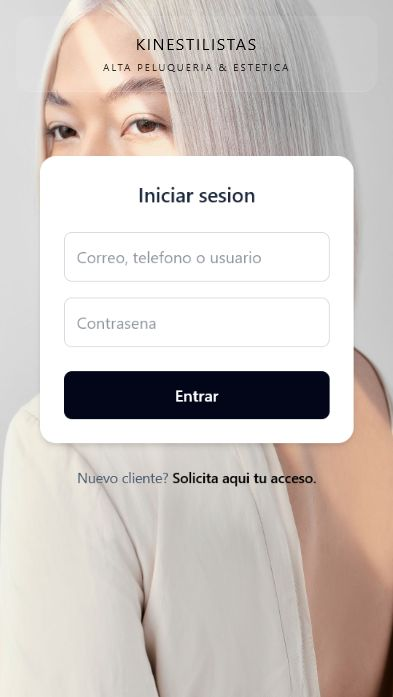
\includegraphics[width=\textwidth]{./figures/Capturas/login.png}
        \caption{Login}
    \end{subfigure}
    \hfill
    \begin{subfigure}[b]{0.30\textwidth}
        \centering
        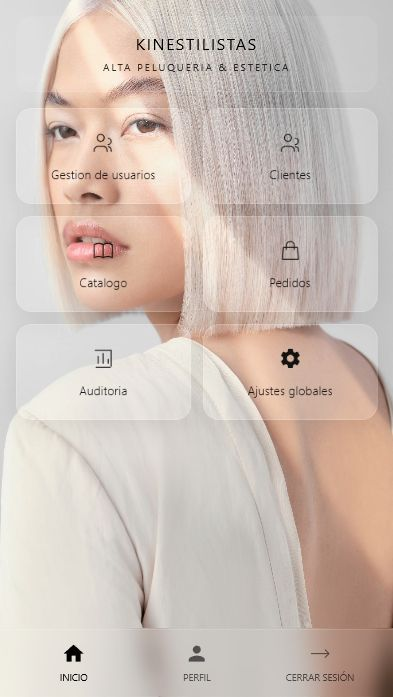
\includegraphics[width=\textwidth]{./figures/Capturas/admin-panel.png}
        \caption{Panel admin}
    \end{subfigure}
    \hfill
    \begin{subfigure}[b]{0.30\textwidth}
        \centering
        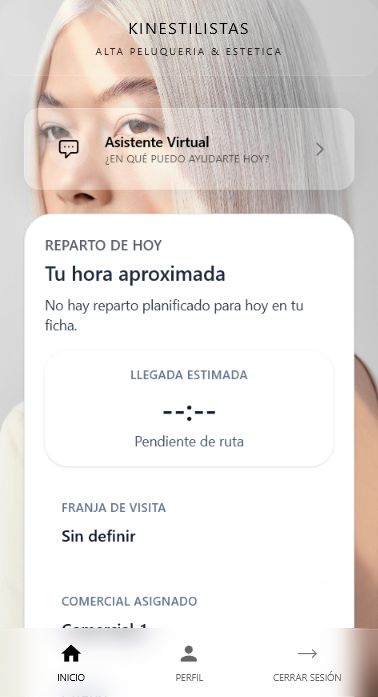
\includegraphics[width=\textwidth]{./figures/Capturas/client-dashboard.png}
        \caption{Vista cliente}
    \end{subfigure}
    \caption{Capturas reales de acceso y paneles por rol}
    \label{fig:ui-real-access-roles}
\end{figure}

\begin{figure}[H]
    \centering
    \begin{subfigure}[b]{0.30\textwidth}
        \centering
        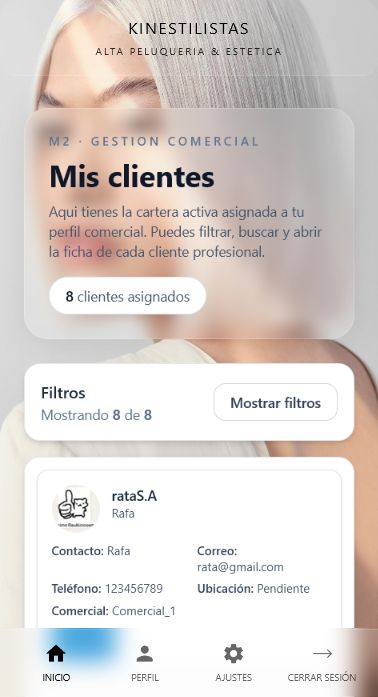
\includegraphics[width=\textwidth]{./figures/Capturas/commercial-clients.png}
        \caption{Clientes}
    \end{subfigure}
    \hfill
    \begin{subfigure}[b]{0.30\textwidth}
        \centering
        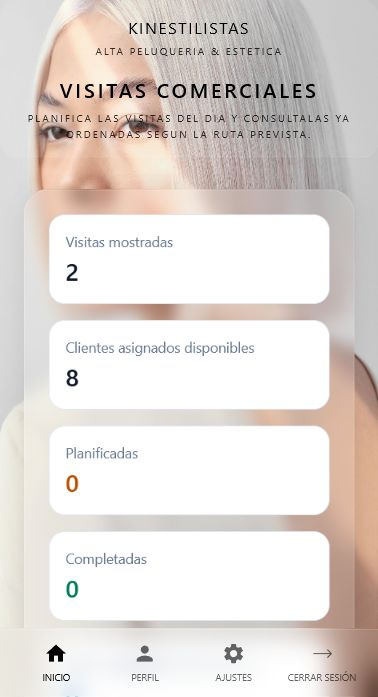
\includegraphics[width=\textwidth]{./figures/Capturas/commercial-visits.png}
        \caption{Visitas}
    \end{subfigure}
    \hfill
    \begin{subfigure}[b]{0.30\textwidth}
        \centering
        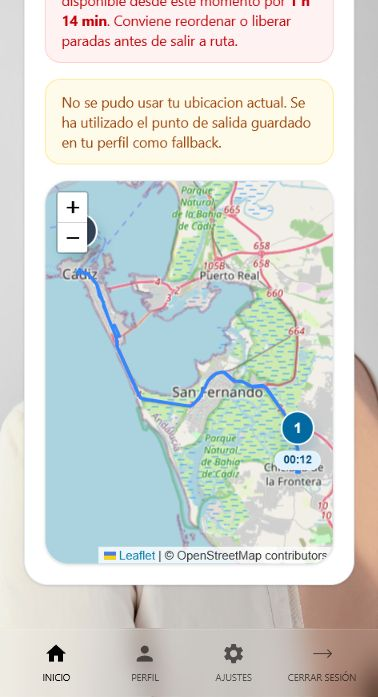
\includegraphics[width=\textwidth]{./figures/Capturas/commercial-routes-map.png}
        \caption{Rutas y mapa}
    \end{subfigure}
    \caption{Capturas reales del espacio comercial}
    \label{fig:ui-real-commercial}
\end{figure}

\begin{figure}[H]
    \centering
    \begin{subfigure}[b]{0.30\textwidth}
        \centering
        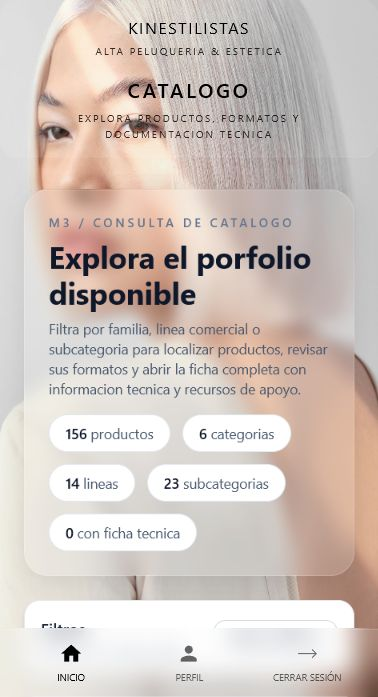
\includegraphics[width=\textwidth]{./figures/Capturas/client-catalog.png}
        \caption{Catálogo}
    \end{subfigure}
    \hfill
    \begin{subfigure}[b]{0.30\textwidth}
        \centering
        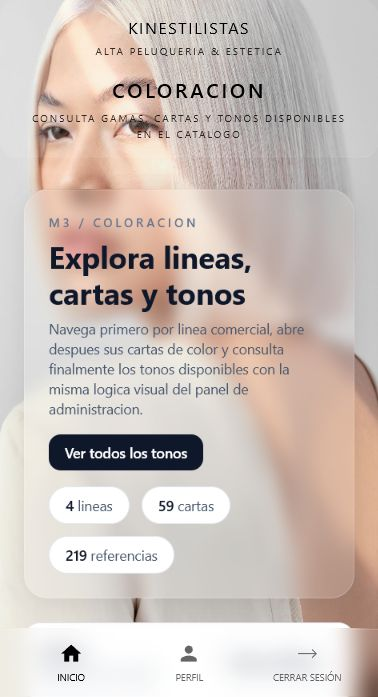
\includegraphics[width=\textwidth]{./figures/Capturas/client-coloration.png}
        \caption{Coloración}
    \end{subfigure}
    \hfill
    \begin{subfigure}[b]{0.30\textwidth}
        \centering
        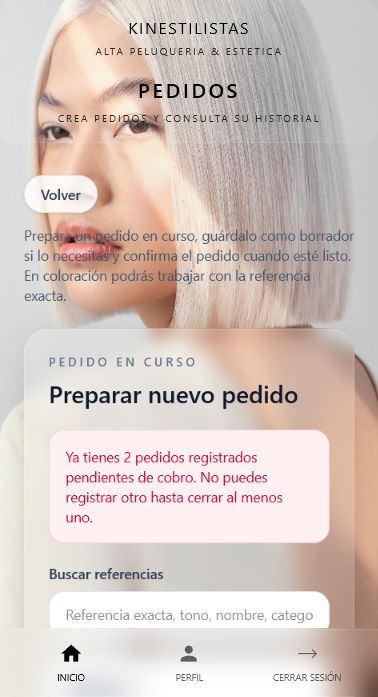
\includegraphics[width=\textwidth]{./figures/Capturas/client-orders.png}
        \caption{Pedidos}
    \end{subfigure}
    \caption{Capturas reales de catálogo, coloración y pedidos}
    \label{fig:ui-real-client-modules}
\end{figure}

Como evidencia visual especifica del modulo \texttt{M6}, se han incorporado tambien capturas del centro administrativo de comunicaciones y de las vistas finales usadas por cliente y comercial. Estas pantallas muestran la publicacion de promociones, el acceso a formaciones, las notificaciones internas y el indicador de avisos pendientes desde los paneles de rol.

\begin{figure}[H]
    \centering
    \begin{subfigure}[b]{0.30\textwidth}
        \centering
        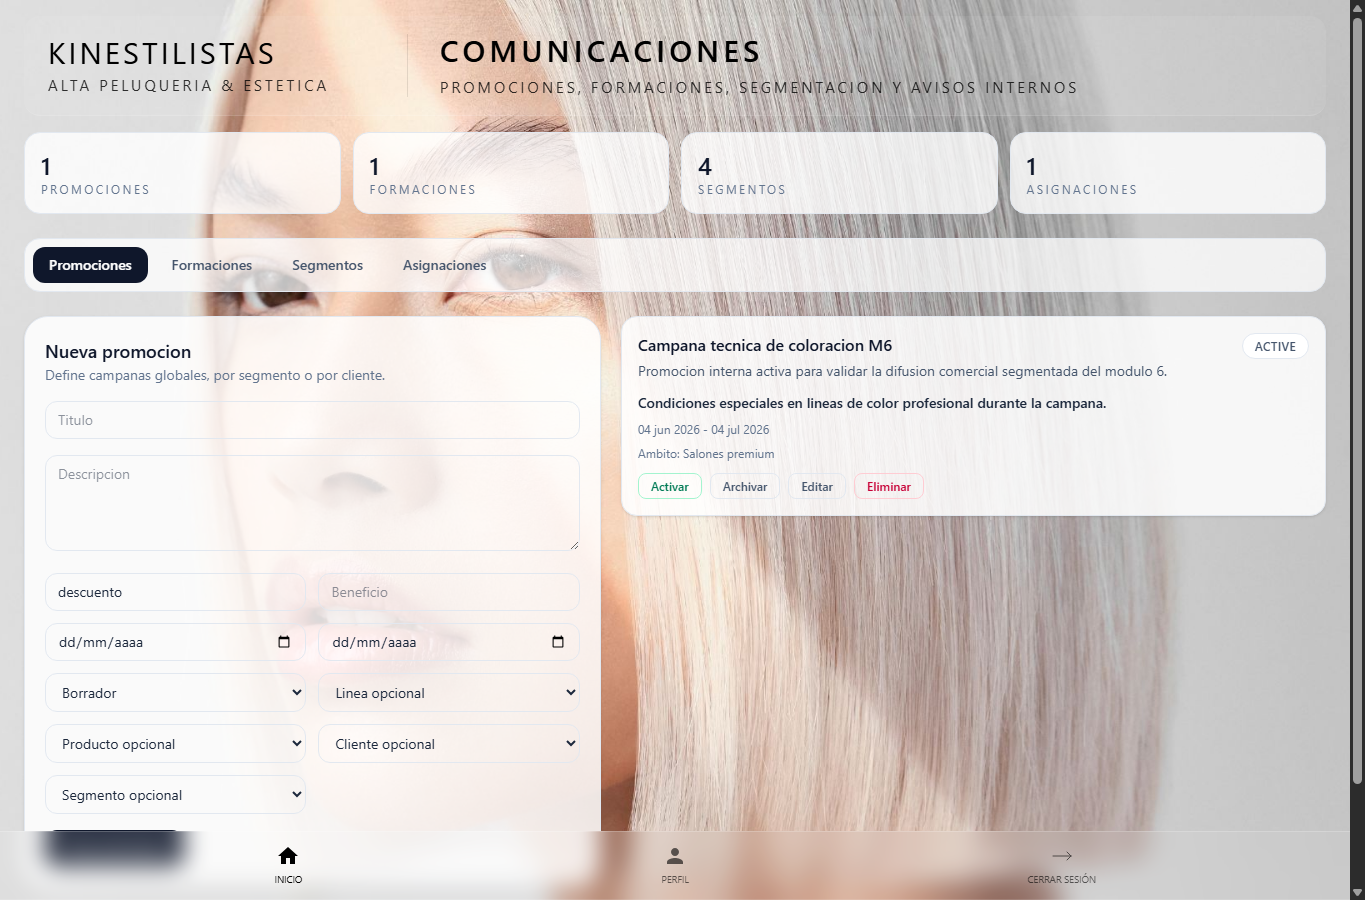
\includegraphics[width=\textwidth]{./figures/Capturas/m6-admin-communications.png}
        \caption{Admin comunicaciones}
    \end{subfigure}
    \hfill
    \begin{subfigure}[b]{0.30\textwidth}
        \centering
        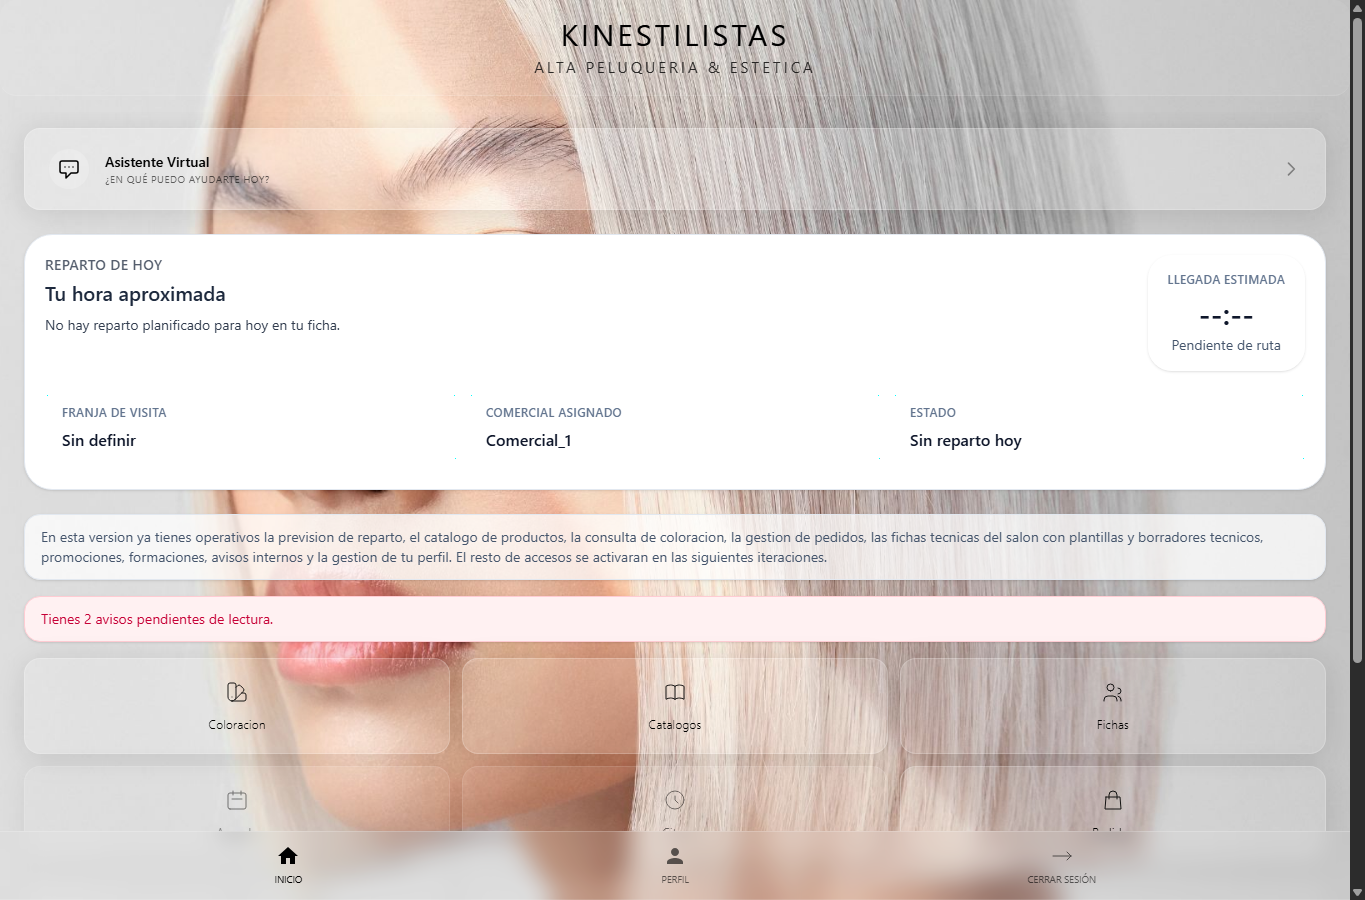
\includegraphics[width=\textwidth]{./figures/Capturas/m6-client-dashboard-notification.png}
        \caption{Panel cliente}
    \end{subfigure}
    \hfill
    \begin{subfigure}[b]{0.30\textwidth}
        \centering
        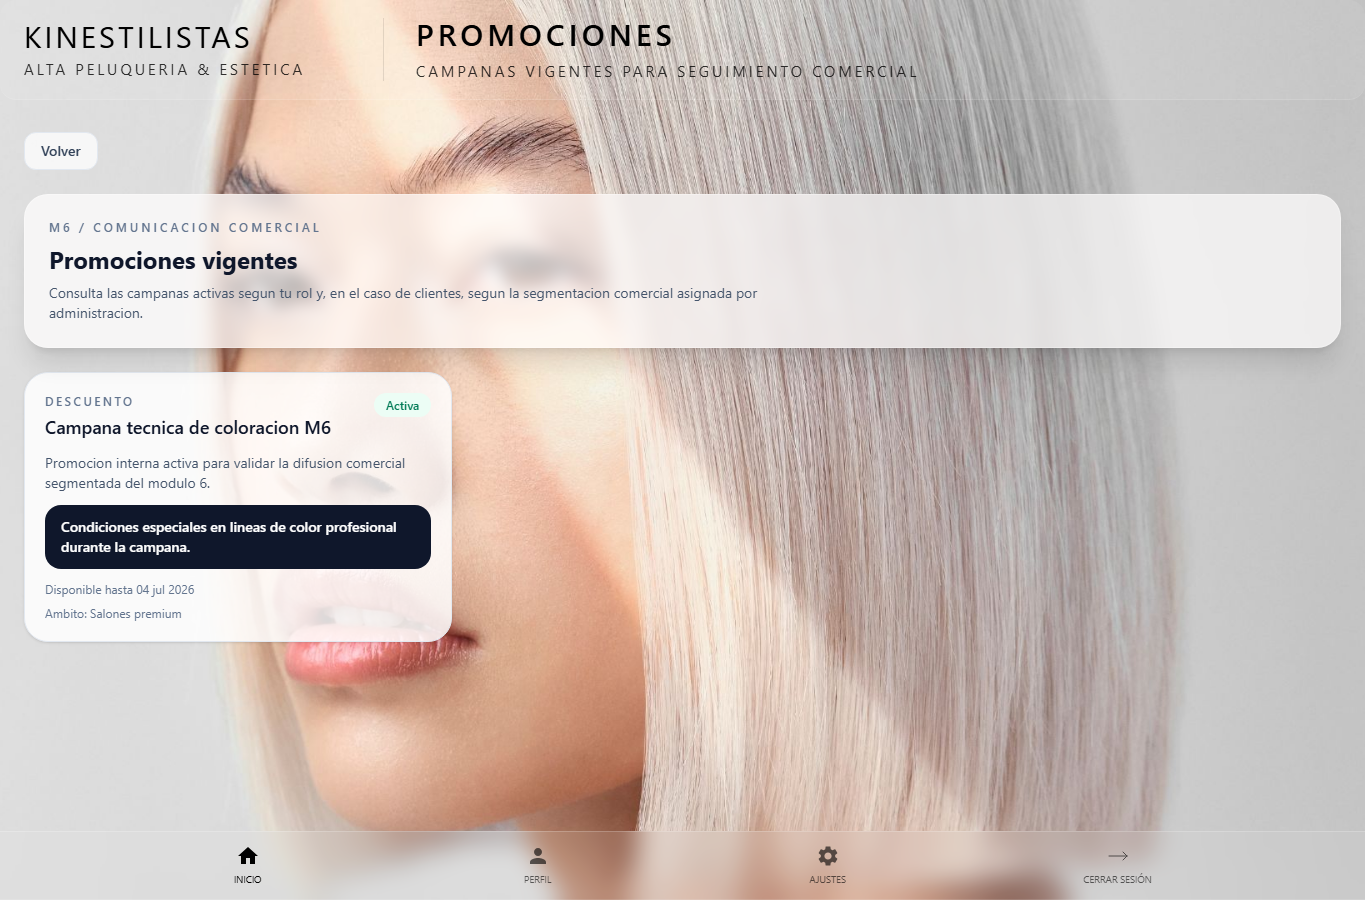
\includegraphics[width=\textwidth]{./figures/Capturas/m6-commercial-promotions.png}
        \caption{Promociones comercial}
    \end{subfigure}
    \caption{Capturas reales del modulo M6 por perfil de usuario}
    \label{fig:ui-real-m6-role-summary}
\end{figure}

\begin{figure}[H]
    \centering
    \begin{subfigure}[b]{0.30\textwidth}
        \centering
        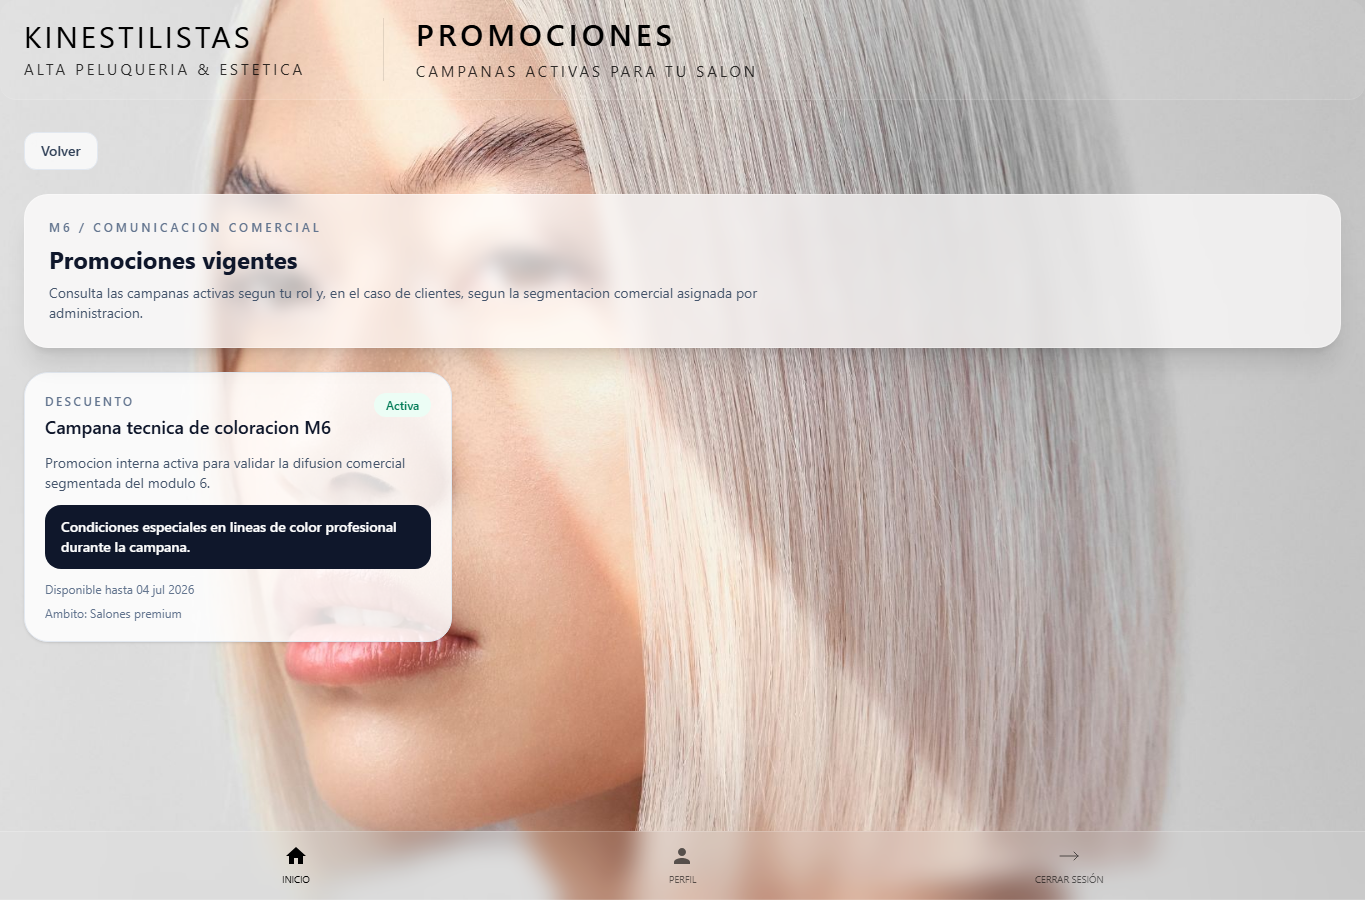
\includegraphics[width=\textwidth]{./figures/Capturas/m6-client-promotions.png}
        \caption{Promociones cliente}
    \end{subfigure}
    \hfill
    \begin{subfigure}[b]{0.30\textwidth}
        \centering
        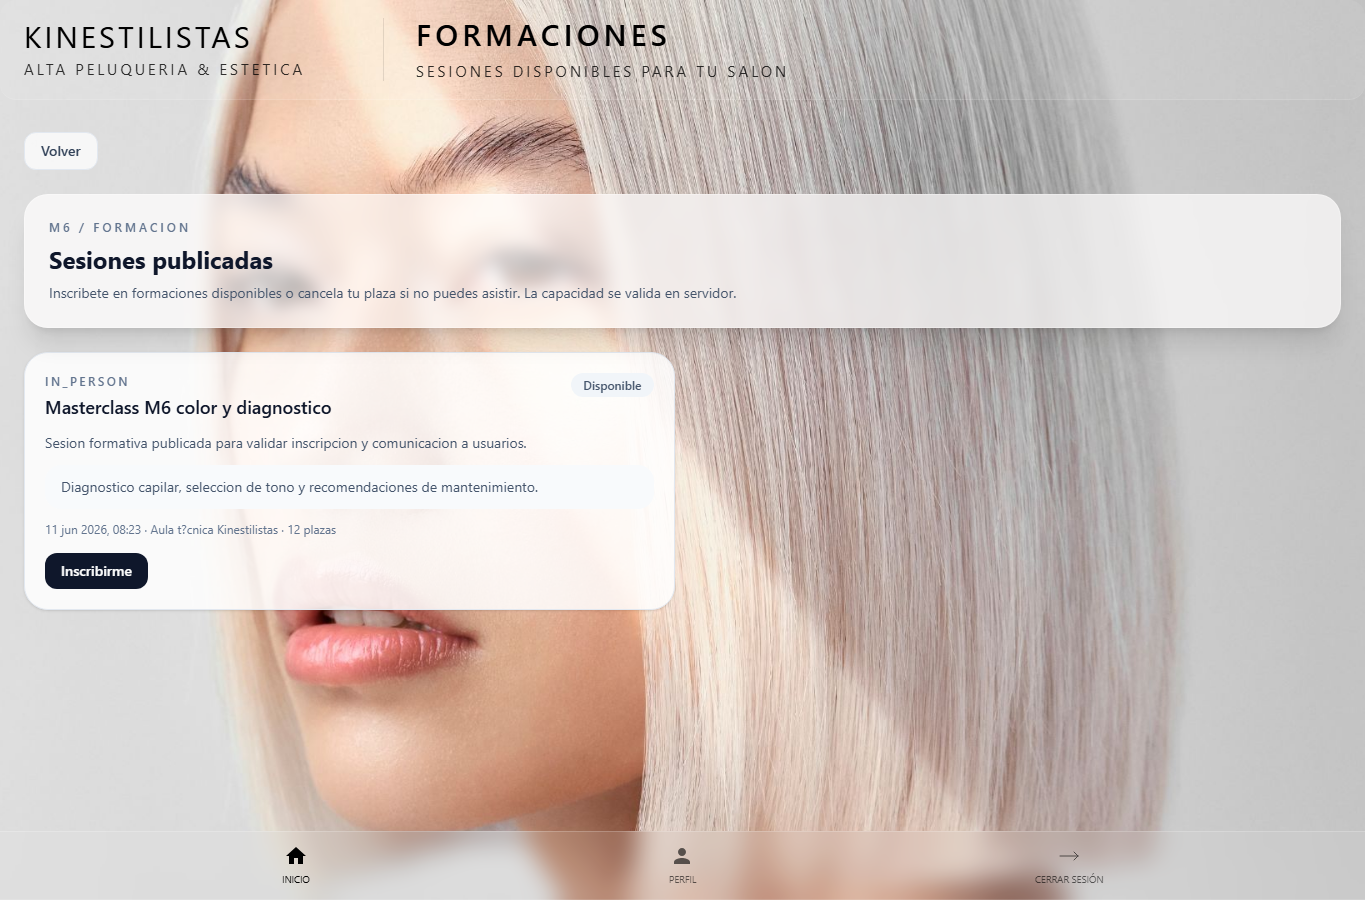
\includegraphics[width=\textwidth]{./figures/Capturas/m6-client-trainings.png}
        \caption{Formaciones}
    \end{subfigure}
    \hfill
    \begin{subfigure}[b]{0.30\textwidth}
        \centering
        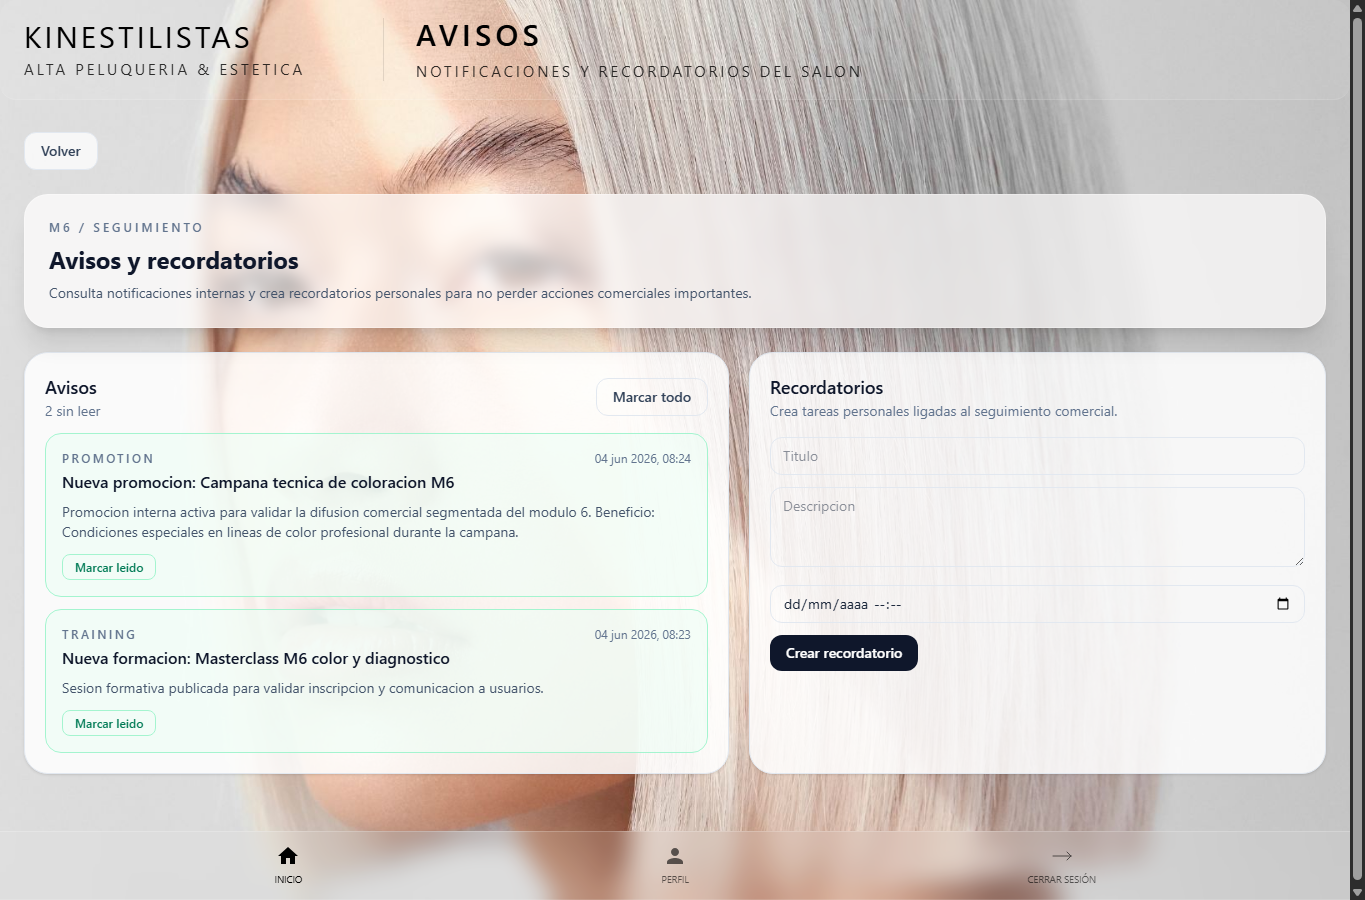
\includegraphics[width=\textwidth]{./figures/Capturas/m6-client-notifications.png}
        \caption{Avisos}
    \end{subfigure}
    \caption{Capturas reales de promociones, formaciones y avisos del modulo M6}
    \label{fig:ui-real-m6-user-flows}
\end{figure}

\section{Modelo de Comportamiento}
El modelo de comportamiento se centra en los flujos que cruzan varias capas de la aplicación y que, por tanto, son especialmente relevantes para verificar la coherencia entre interfaz, autenticación, servicios de dominio y persistencia.

\begin{figure}[H]
    \centering
    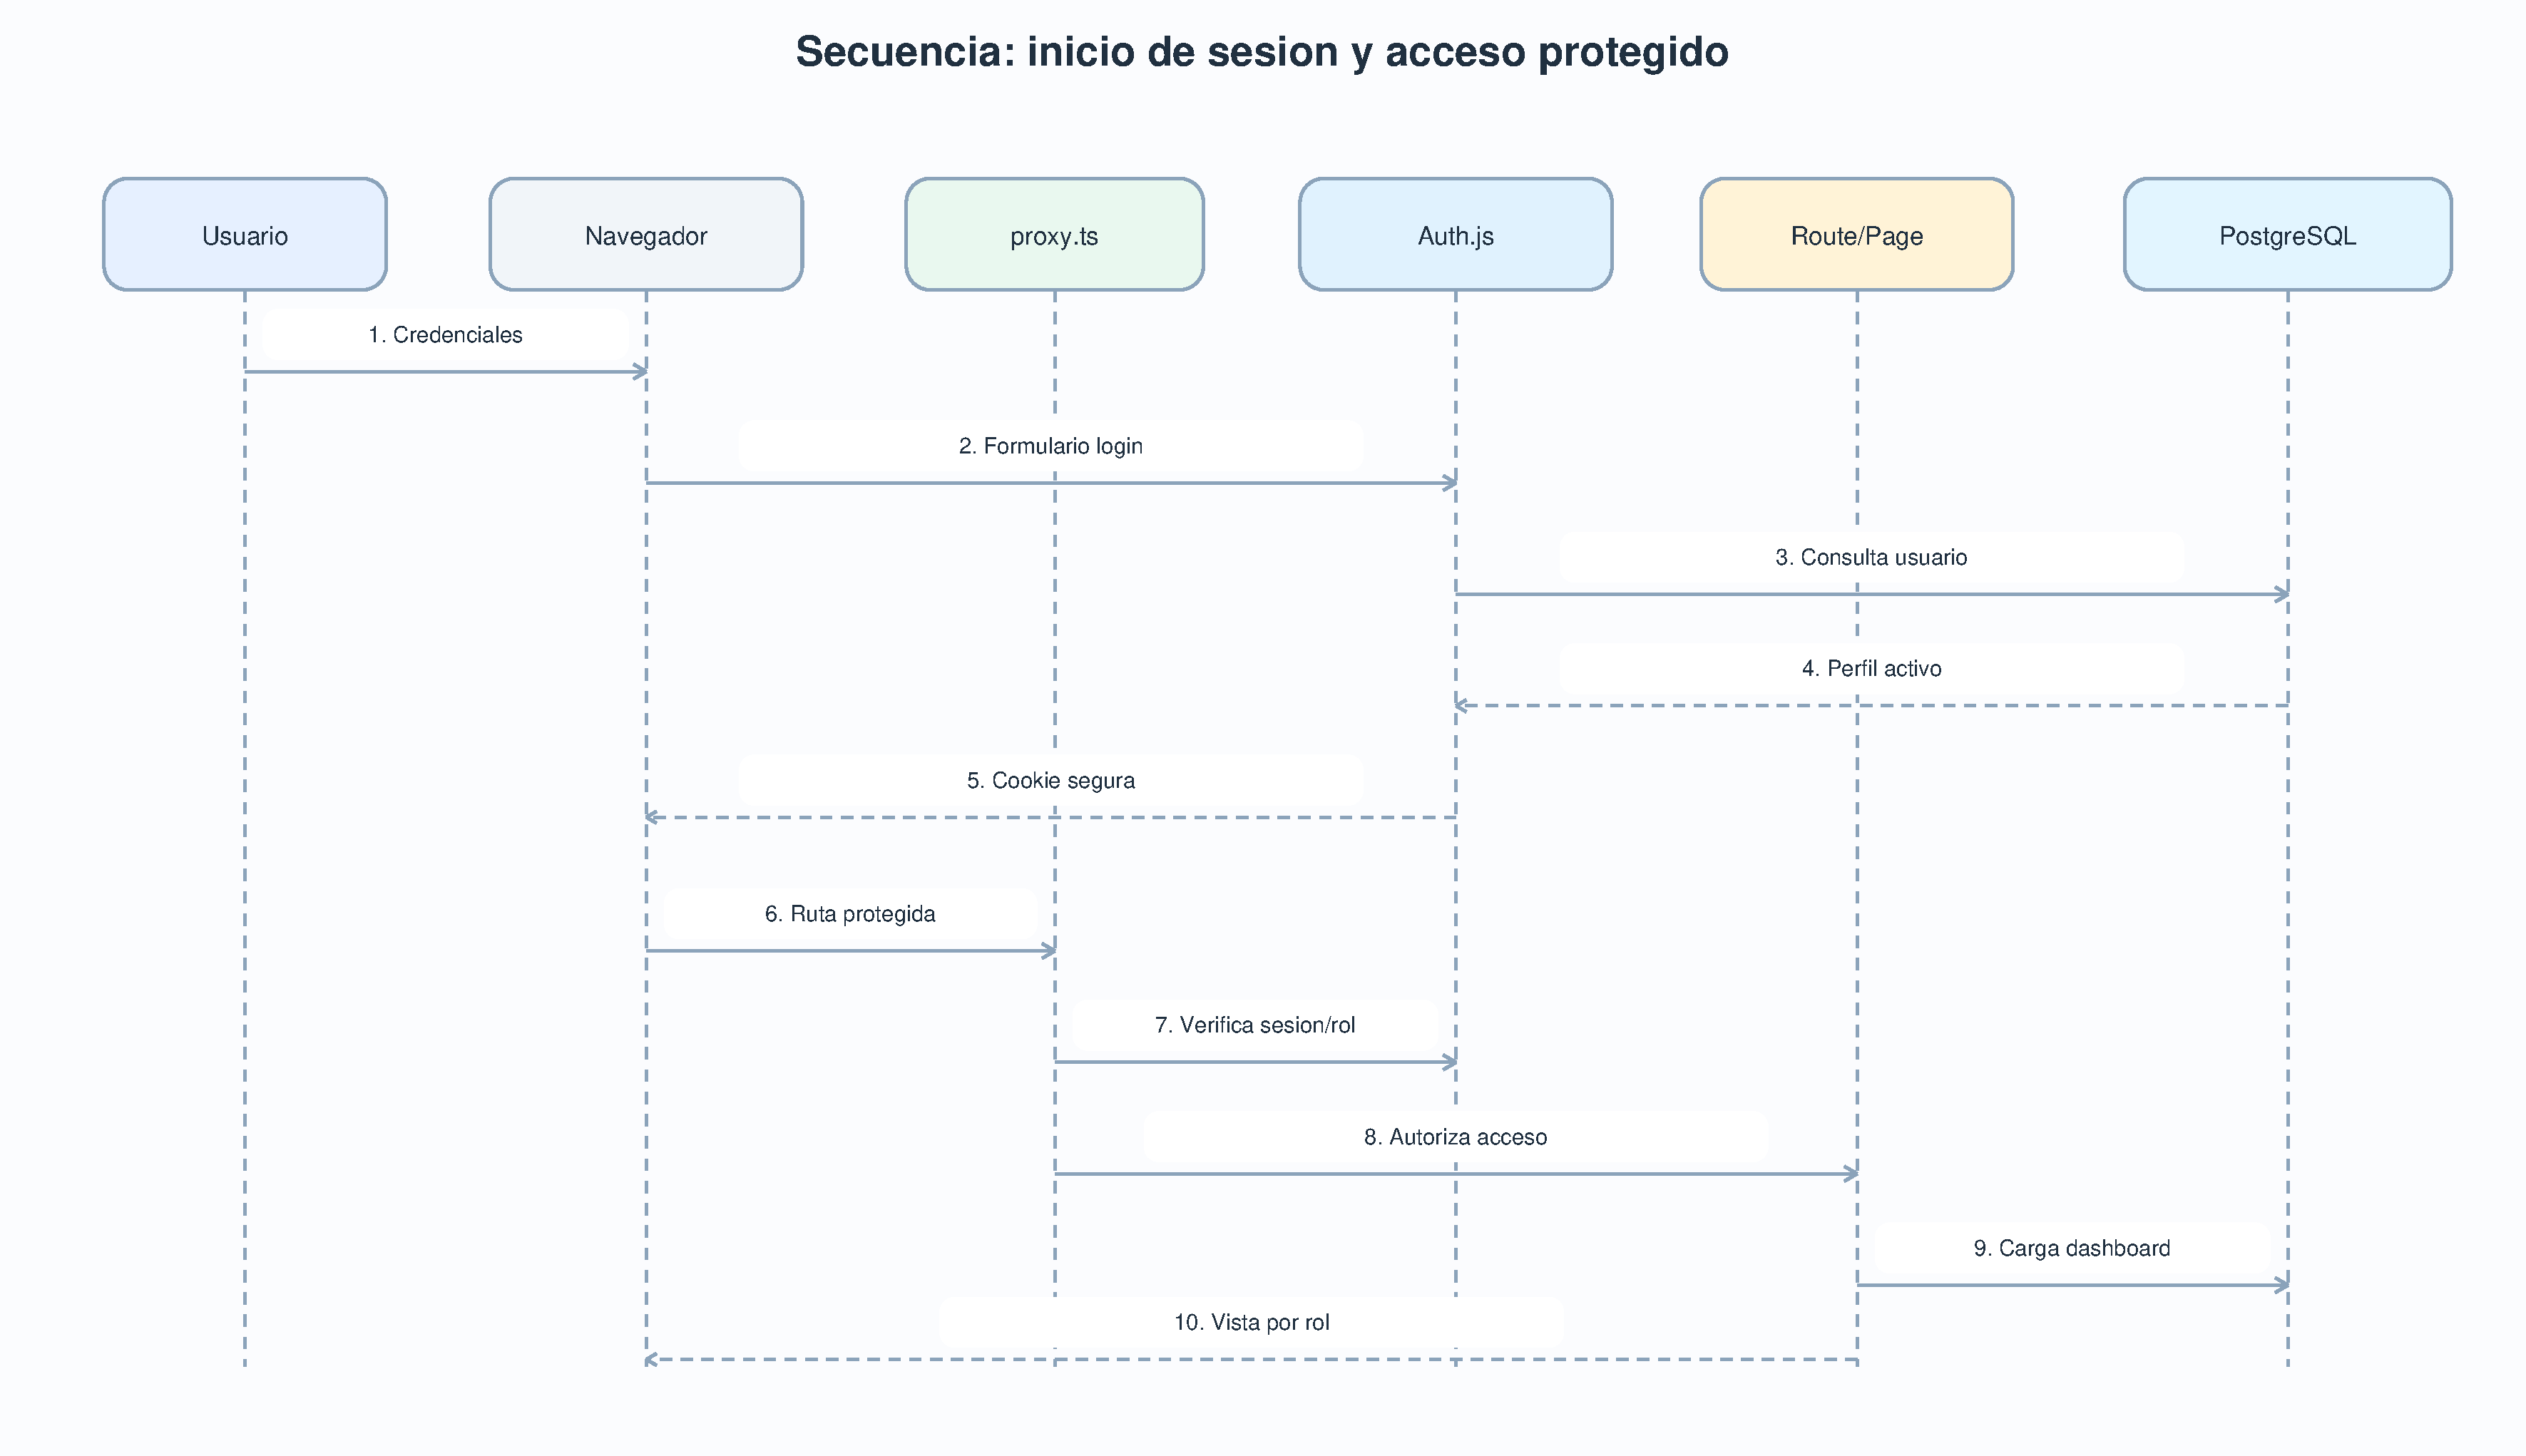
\includegraphics[width=\textwidth]{./figures/UML/Secuencia/sequence-login-protected-access.pdf}
    \caption{Diagrama de secuencia: inicio de sesión y acceso protegido}
    \label{fig:seq-login-protected-access}
\end{figure}

La Figura~\ref{fig:seq-login-protected-access} resume el acceso al sistema: el usuario introduce credenciales, \texttt{Auth.js} valida la identidad contra \texttt{PostgreSQL}, se genera una cookie de sesión segura y \texttt{proxy.ts} controla el acceso posterior a rutas protegidas.

\begin{figure}[H]
    \centering
    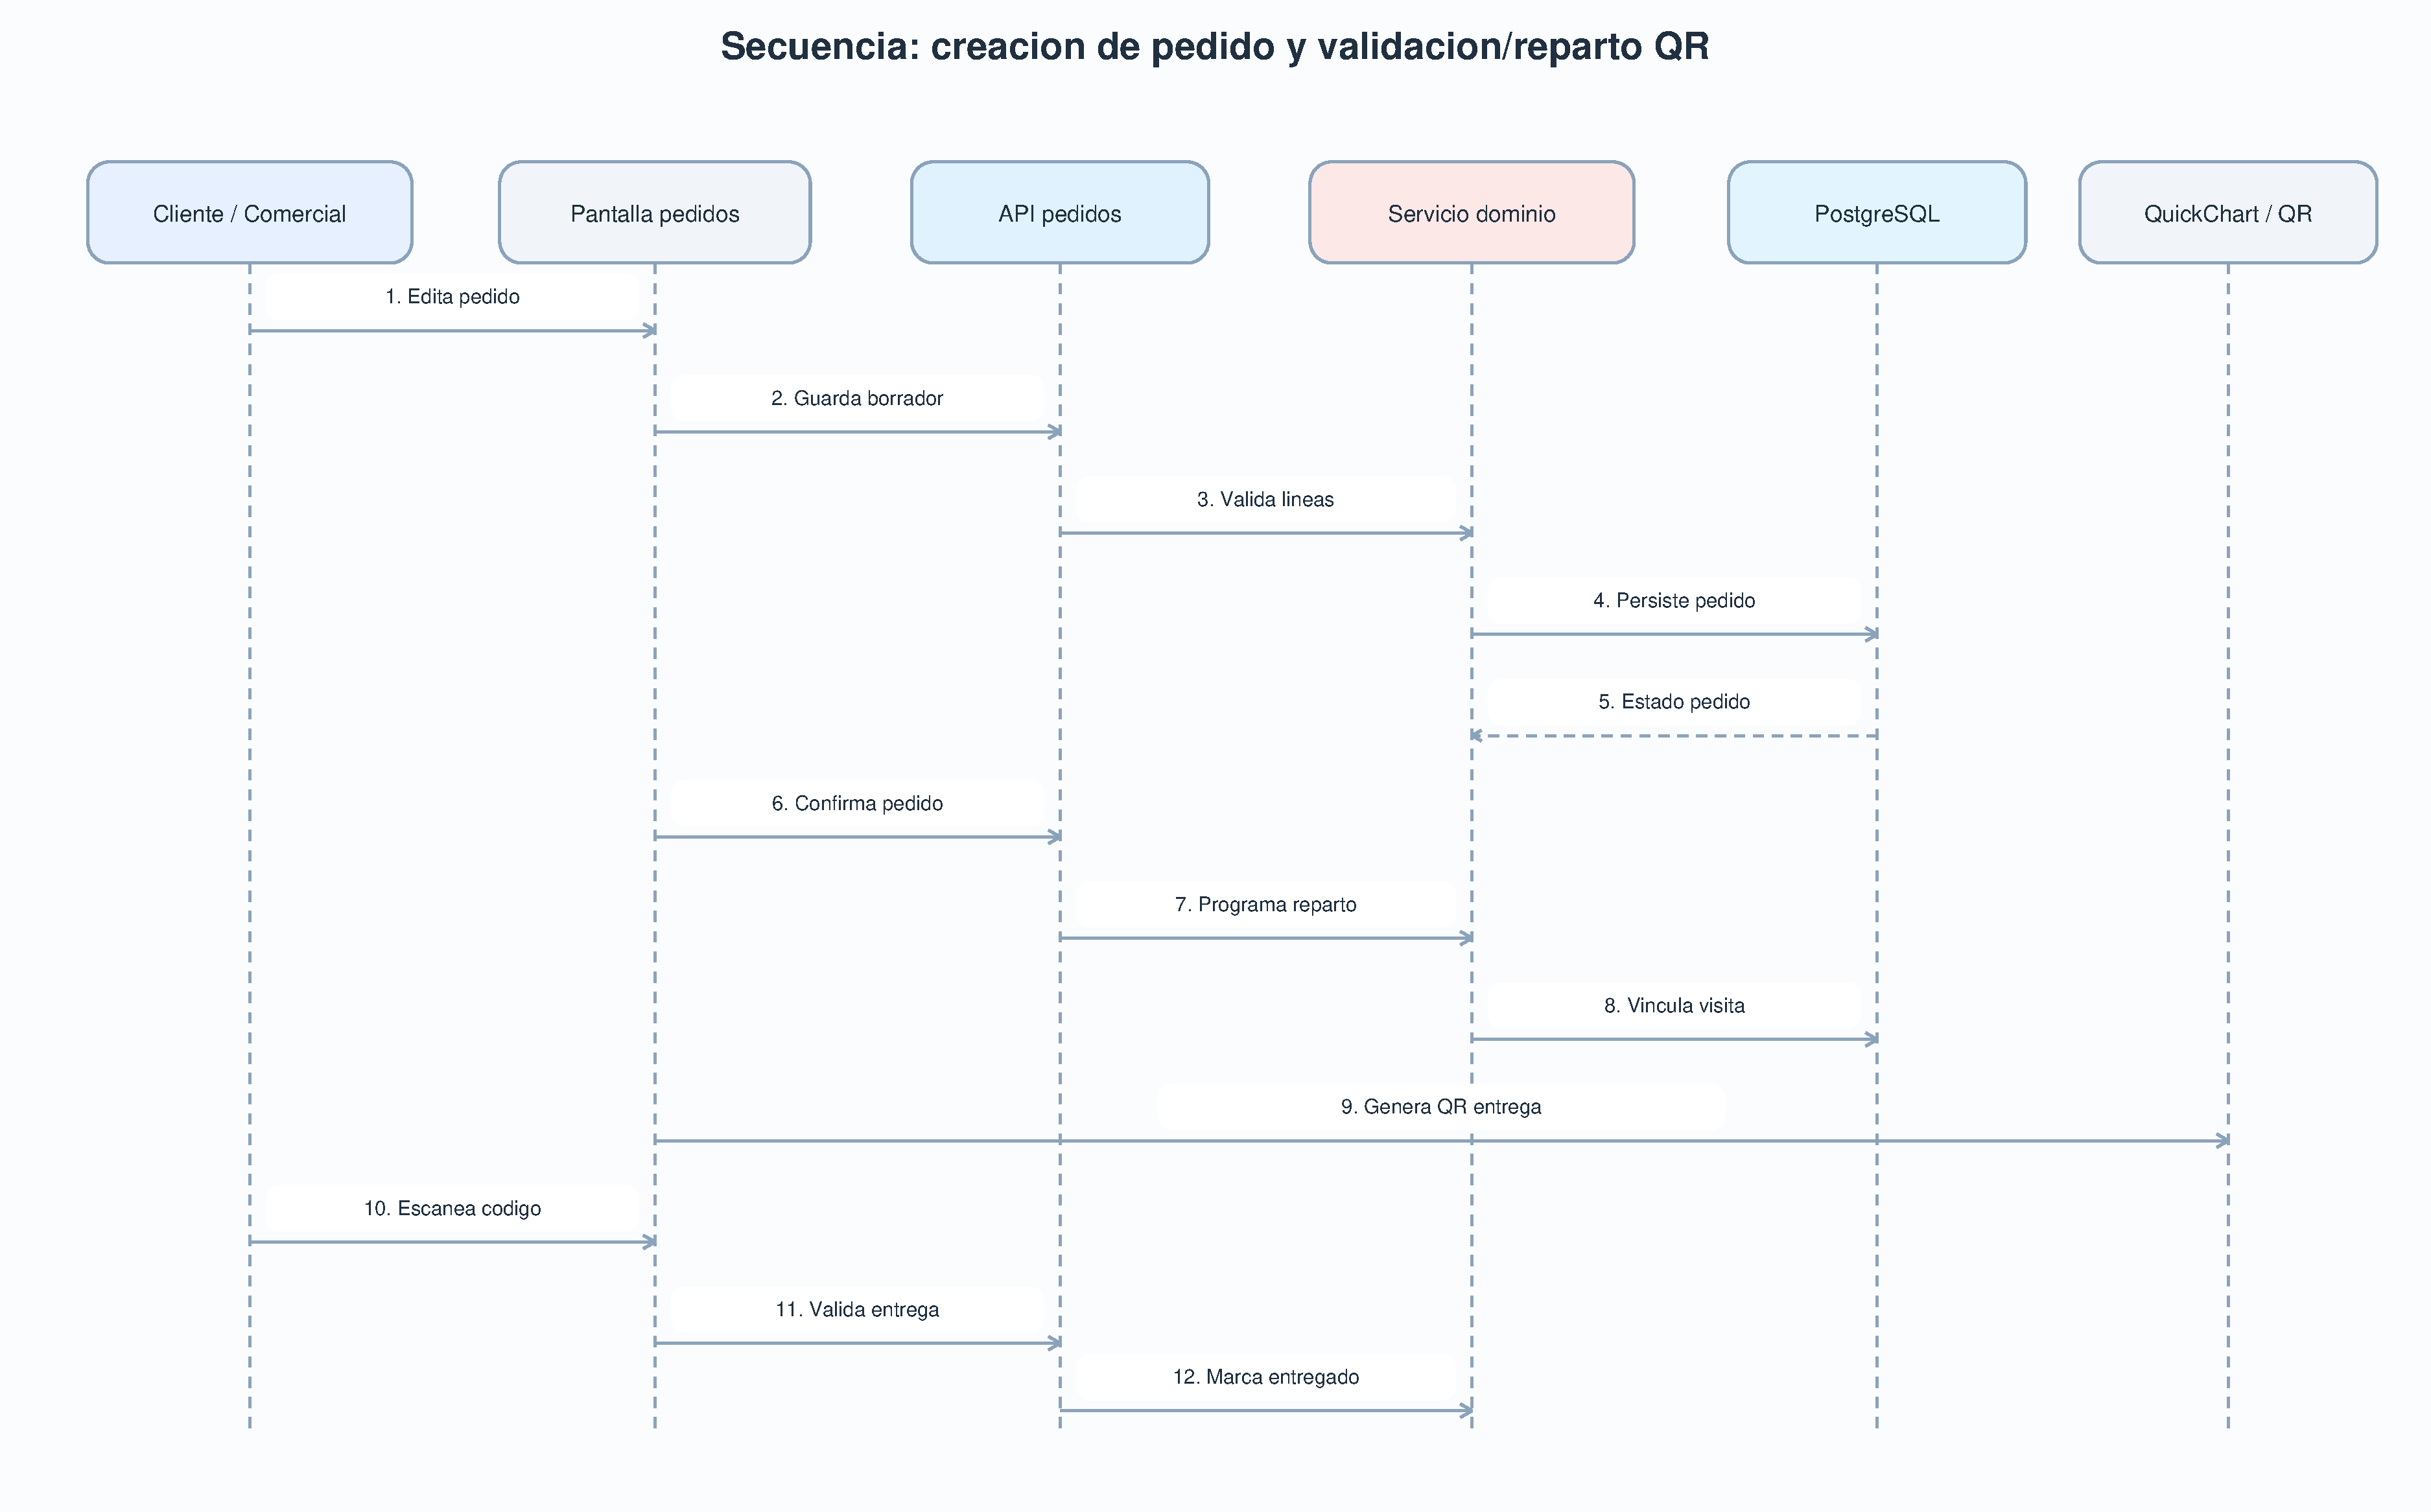
\includegraphics[width=\textwidth]{./figures/UML/Secuencia/sequence-order-qr-delivery.pdf}
    \caption{Diagrama de secuencia: creación de pedido y validación/reparto QR}
    \label{fig:seq-order-qr-delivery}
\end{figure}

La Figura~\ref{fig:seq-order-qr-delivery} recoge el flujo de pedido y reparto: la pantalla de pedidos registra líneas, la API valida productos y tonos, el servicio de dominio persiste el pedido, se vincula la entrega a una visita comercial y el QR permite confirmar la entrega desde el detalle operativo.
